\section{Casi d'uso}
\subsection{Introduzione}
In questa sezione del documento vengono analizzati nel dettaglio i casi d'uso individuati per il sistema.
nel corso dell'analisi del \href{https://7last.github.io/docs/rtb/documentazione-interna/glossario\#capitolato}{capitolato\textsubscript{G}} e dei colloqui con la \href{https://7last.github.io/docs/rtb/documentazione-interna/glossario\#proponente}{proponente\textsubscript{G}}.

\subsection{Struttura dei casi d'uso}
In tutto il documento ci si riferirà ai casi d'uso utilizzando la sigla \texttt{UC} seguita dal rispettivo codice nella forma
\begin{center}
	\textbf{UC-[identificativo\_caso\_principale].[identificativo\_sotto\_caso]}
\end{center}

il quale permette di utilizzarlo come riferimento in questo e altri documenti.\\
Per ciascun caso d'uso vengono definiti i seguenti elementi:
\begin{itemize}
	\item \textbf{Attore principale}: l'attore primariamente coinvolto nel caso d'uso;
	\item \textbf{Precondizioni}: le condizioni che devono essere verificate affinché il caso d'uso possa essere
	      eseguito;
	\item \textbf{Postcondizioni}: le condizioni che devono essere verificate al termine dell'esecuzione del caso
	\item \textbf{Scenario principale}: la sequenza di passi che descrive il comportamento del sistema durante
	      l'esecuzione del caso d'uso;
	\item \href{https://7last.github.io/docs/rtb/documentazione-interna/glossario\#user-story}{\textbf{User story}\textsubscript{G}}: una descrizione testuale del caso d'uso.
\end{itemize}


\subsection{Attori}
I seguenti attori sono coinvolti nei casi d'uso:
\begin{itemize}
	\item Impiegati presso \textbf{autorità locali}: essi possono accedere al sistema per visualizzare i dati
	      monitoraggio della \href{https://7last.github.io/docs/rtb/documentazione-interna/glossario\#smart-city}{\textit{Smart City}\textsubscript{G}}.
	\item \textbf{Sensori}: sorgente di dati con un determinato dominio di interesse che effettua misurazioni
	      e trasmette i dati al sistema.
\end{itemize}

\subsection{Elenco dei casi d'uso}
\subsubsection{UC-1: Visualizzazione dashboard generale}
\begin{itemize}
	\item \textbf{Attore principale}: Autorità locale;
	\item \textbf{Precondizioni}: L'autorità locale ha effettuato l'accesso al sistema ed esso è in funzione;
	\item \textbf{Postcondizioni}: L'autorità locale visualizza la \href{https://7last.github.io/docs/rtb/documentazione-interna/glossario\#dashboard}{dashboard\textsubscript{G}} generale con i dati relativi ai sensori;
	      presenti nella città;
	\item \textbf{Scenario principale}:
	      \begin{enumerate}
		      \item L'autorità locale accede alla piattaforma;
		      \item Il sistema carica i dati trasmessi dai sensori interrogando il database.
	      \end{enumerate}
	\item \href{https://7last.github.io/docs/rtb/documentazione-interna/glossario\#user-story}{\textbf{User story}\textsubscript{G}}: Come autorità locale desidero poter visualizzare una \href{https://7last.github.io/docs/rtb/documentazione-interna/glossario\#dashboard}{dashboard\textsubscript{G}} generale con i dati relativi ai sensori presenti,
	      la quale mi consente di monitorare in tempo reale lo stato della città ed eventualmente prendere decisioni.
\end{itemize}

\begin{center}
	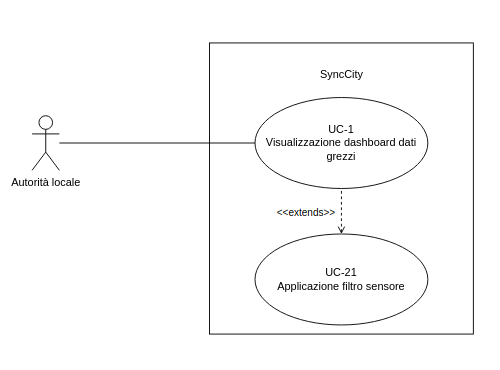
\includegraphics[width=0.6\textwidth]{analisi_dei_requisiti/UC-1.png}
	\captionof{figure}{UC-1: Visualizzazione \href{https://7last.github.io/docs/rtb/documentazione-interna/glossario\#dashboard}{dashboard\textsubscript{G}} generale}
\end{center}

\subsubsubsection{UC-1.1: Visualizzazione mappa interattiva sensori}
\begin{itemize}
	\item \textbf{Attore principale}: Autorità locale;
	\item \textbf{Precondizioni}: L'autorità locale ha effettuato l'accesso al sistema ed esso è in funzione;
	\item \textbf{Postcondizioni}: L'autorità locale visualizza un \textit{panel} contenente una mappa interattiva
	      popolata con dei marker rappresentanti la posizione dei sensori;
	\item \textbf{Scenario principale}:
	      \begin{enumerate}
		      \item L'autorità locale accede alla piattaforma;
		      \item Il sistema carica i dati trasmessi dai sensori interrogando il database;
		      \item L'autorità locale seleziona la visualizzazione della \href{https://7last.github.io/docs/rtb/documentazione-interna/glossario\#dashboard}{dashboard\textsubscript{G}} generale.
	      \end{enumerate}
	\item \href{https://7last.github.io/docs/rtb/documentazione-interna/glossario\#user-story}{\textbf{User story}\textsubscript{G}}: Come autorità locale desidero poter visualizzare una mappa interattiva popolata con dei marker rappresentanti
	      la posizione dei sensori e contenenti il loro identificativo. Essa mi consentirà di visualizzare la distribuzione dei sensori nel territorio.
\end{itemize}

\begin{center}
	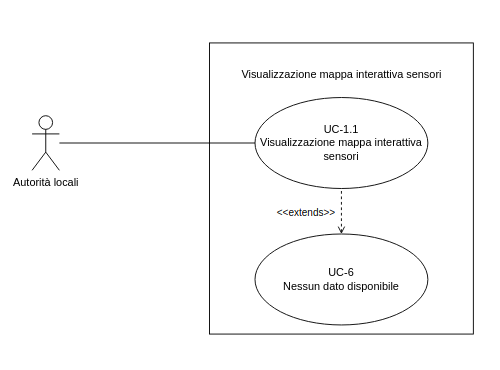
\includegraphics[width=0.6\textwidth]{analisi_dei_requisiti/UC-1.1.png}
	\captionof{figure}{UC-1.1: Visualizzazione mappa interattiva sensori}
\end{center}

\subsubsubsection{UC-1.2: Visualizzazione tabella sensori}
\begin{itemize}
	\item \textbf{Attore principale}: Autorità locale;
	\item \textbf{Precondizioni}: L'autorità locale ha effettuato l'accesso al sistema ed esso è in funzione;
	\item \textbf{Postcondizioni}: L'autorità locale visualizza un \textit{panel} contenente una tabella contenente tutti i sensori collegati al sistema;
	\item \textbf{Scenario principale}:
	      \begin{enumerate}
		      \item L'autorità locale accede alla piattaforma;
		      \item Il sistema carica i dati relativi ai sensori interrogando il database;
		      \item L'autorità locale seleziona la visualizzazione della \href{https://7last.github.io/docs/rtb/documentazione-interna/glossario\#dashboard}{dashboard\textsubscript{G}} generale.
	      \end{enumerate}
	\item \href{https://7last.github.io/docs/rtb/documentazione-interna/glossario\#user-story}{\textbf{User story}\textsubscript{G}}: Come autorità locale desidero poter visualizzare una tabella contenente una tabella contenente tutti i sensori collegati al sistema,
	      contenente l'identificativo del \href{https://7last.github.io/docs/rtb/documentazione-interna/glossario\#sensore}{sensore\textsubscript{G}}, la sua tipologia, posizione e data di ultima trasmissione.
\end{itemize}

\begin{center}
	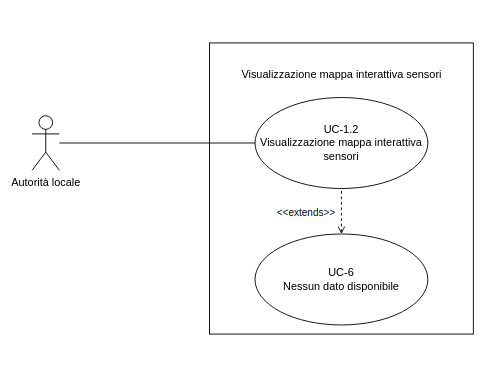
\includegraphics[width=0.6\textwidth]{analisi_dei_requisiti/UC-1.2.png}
	\captionof{figure}{UC-1.2: Visualizzazione tabella sensori}
\end{center}

\subsubsection{UC-2: Visualizzazione dashboard dati atmosferici}
\begin{itemize}
	\item \textbf{Attore principale}: Autorità locale;
	\item \textbf{Precondizioni}: L'autorità locale ha effettuato l'accesso al sistema ed esso è in funzione;
	\item \textbf{Postcondizioni}: L'autorità locale visualizza una \href{https://7last.github.io/docs/rtb/documentazione-interna/glossario\#dashboard}{dashboard\textsubscript{G}} contenente i \href{https://7last.github.io/docs/rtb/documentazione-interna/glossario\#dati-atmosferici}{dati atmosferici\textsubscript{G}} provenienti dai sensori;
	\item \textbf{Scenario principale}:
	      \begin{enumerate}
		      \item L'autorità locale accede alla piattaforma;
		      \item Il sistema carica i dati relativi ai sensori di \href{https://7last.github.io/docs/rtb/documentazione-interna/glossario\#dati-atmosferici}{dati atmosferici\textsubscript{G}} interrogando il database.
	      \end{enumerate}
	\item \href{https://7last.github.io/docs/rtb/documentazione-interna/glossario\#user-story}{\textbf{User story}\textsubscript{G}}: Come autorità locale desidero poter visualizzare una \href{https://7last.github.io/docs/rtb/documentazione-interna/glossario\#dashboard}{dashboard\textsubscript{G}} relativa ai \href{https://7last.github.io/docs/rtb/documentazione-interna/glossario\#dati-atmosferici}{dati atmosferici\textsubscript{G}}
	      la quale mi deve consentire di visualizzare i dati storici e in tempo reale. Tale \href{https://7last.github.io/docs/rtb/documentazione-interna/glossario\#dashboard}{dashboard\textsubscript{G}} contiene misurazioni di temperatura,
	      pressione, umidità, precipitazioni...
\end{itemize}

\begin{center}
	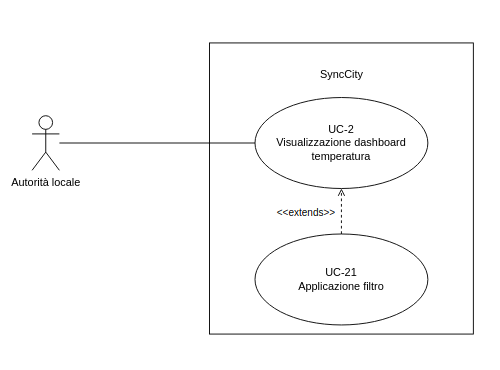
\includegraphics[width=0.6\textwidth]{analisi_dei_requisiti/UC-2.png}
	\captionof{figure}{UC-2: Visualizzazione \href{https://7last.github.io/docs/rtb/documentazione-interna/glossario\#dashboard}{dashboard\textsubscript{G}} \href{https://7last.github.io/docs/rtb/documentazione-interna/glossario\#dati-atmosferici}{dati atmosferici\textsubscript{G}}}
\end{center}

% temperatura
\subsubsubsection{UC-2.1: Visualizzazione grafico time series per temperatura}
\begin{itemize}
	\item \textbf{Attore principale}: Autorità locale;
	\item \textbf{Precondizioni}:
	      \begin{enumerate}
		      \item L'autorità locale ha effettuato l'accesso al sistema ed esso è in funzione;
		      \item Il sistema ha caricato la \href{https://7last.github.io/docs/rtb/documentazione-interna/glossario\#dashboard}{dashboard\textsubscript{G}} relativa ai \href{https://7last.github.io/docs/rtb/documentazione-interna/glossario\#dati-atmosferici}{dati atmosferici\textsubscript{G}};
	      \end{enumerate}


	\item \textbf{Postcondizioni}: L'autorità locale visualizza un grafico \href{https://7last.github.io/docs/rtb/documentazione-interna/glossario\#time-series}{time series\textsubscript{G}} contenente le misurazioni storiche
	      della temperatura;
	\item \textbf{Scenario principale}:
	      \begin{enumerate}
		      \item L'autorità locale accede alla piattaforma;
		      \item Il sistema carica i dati relativi ai sensori interrogando il database;
		      \item L'autorità locale seleziona la visualizzazione della \href{https://7last.github.io/docs/rtb/documentazione-interna/glossario\#dashboard}{dashboard\textsubscript{G}} relativa ai \href{https://7last.github.io/docs/rtb/documentazione-interna/glossario\#dati-atmosferici}{dati atmosferici\textsubscript{G}}.
	      \end{enumerate}
	\item \href{https://7last.github.io/docs/rtb/documentazione-interna/glossario\#user-story}{\textbf{User story}\textsubscript{G}}: Come autorità locale desidero poter visualizzare un grafico \href{https://7last.github.io/docs/rtb/documentazione-interna/glossario\#time-series}{time series\textsubscript{G}} contenente le misurazioni storiche della temperatura
	      per poter monitorarne l'andamento nel tempo e facilmente individuare eventuali anomalie.
\end{itemize}

\begin{center}
	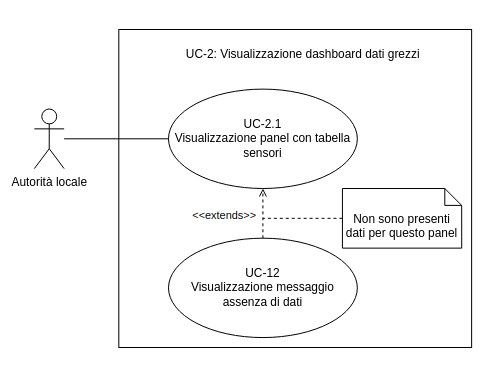
\includegraphics[width=0.75\textwidth]{analisi_dei_requisiti/UC-2.1.png}
	\captionof{figure}{UC-2.1: Visualizzazione grafico \href{https://7last.github.io/docs/rtb/documentazione-interna/glossario\#time-series}{time series\textsubscript{G}} per temperatura}
\end{center}
\subsubsubsection{UC-2.2: Visualizzazione \textit{panel} temperatura in tempo reale}
\begin{itemize}
	\item \textbf{Attore principale}: Autorità locale;
	\item \textbf{Precondizioni}:
	      \begin{enumerate}
		      \item L'autorità locale ha effettuato l'accesso al sistema ed esso è in funzione;
		      \item Il sistema ha caricato la \href{https://7last.github.io/docs/rtb/documentazione-interna/glossario\#dashboard}{dashboard\textsubscript{G}} relativa ai \href{https://7last.github.io/docs/rtb/documentazione-interna/glossario\#dati-atmosferici}{dati atmosferici\textsubscript{G}};
	      \end{enumerate}
	\item \textbf{Postcondizioni}: L'autorità locale visualizza un \textit{panel} contenente la temperatura in tempo reale;
	\item \textbf{Scenario principale}:
	      \begin{enumerate}
		      \item L'autorità locale accede alla piattaforma;
		      \item Il sistema carica i dati relativi ai sensori interrogando il database;
		      \item L'autorità locale seleziona la visualizzazione della \href{https://7last.github.io/docs/rtb/documentazione-interna/glossario\#dashboard}{dashboard\textsubscript{G}} relativa ai \href{https://7last.github.io/docs/rtb/documentazione-interna/glossario\#dati-atmosferici}{dati atmosferici\textsubscript{G}}.
	      \end{enumerate}
	\item \href{https://7last.github.io/docs/rtb/documentazione-interna/glossario\#user-story}{\textbf{User story}\textsubscript{G}}: Come autorità locale desidero poter visualizzare la temperatura in tempo reale per poter monitorare
	      l'andamento della temperatura in tempo reale e prendere decisioni in base ad esso.
\end{itemize}

\begin{center}
	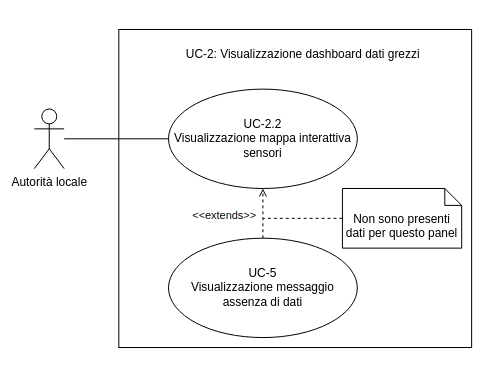
\includegraphics[width=0.75\textwidth]{analisi_dei_requisiti/UC-2.2.png}
	\captionof{figure}{UC-2.2: Visualizzazione \textit{panel} temperatura in tempo reale}
\end{center}

\subsubsubsection{UC-2.3: Visualizzazione \textit{panel} temperatura media}
\begin{itemize}
	\item \textbf{Attore principale}: Autorità locale;
	\item \textbf{Precondizioni}: 	\item \textbf{Postcondizioni}: L'autorità locale visualizza un \textit{panel} contenente la temperatura media in un determinato periodo di tempo;
	      \begin{enumerate}
		      \item L'autorità locale ha effettuato l'accesso al sistema ed esso è in funzione;
		      \item Il sistema ha caricato la \href{https://7last.github.io/docs/rtb/documentazione-interna/glossario\#dashboard}{dashboard\textsubscript{G}} relativa ai \href{https://7last.github.io/docs/rtb/documentazione-interna/glossario\#dati-atmosferici}{dati atmosferici\textsubscript{G}};
	      \end{enumerate}
	\item \textbf{Postcondizioni}: L'autorità locale visualizza un \textit{panel} contenente la temperatura media in un determinato periodo di tempo;
	\item \textbf{Scenario principale}:
	      \begin{enumerate}
		      \item L'autorità locale accede alla piattaforma;
		      \item Il sistema carica i dati relativi ai sensori interrogando il database;
		      \item L'autorità locale seleziona la visualizzazione della \href{https://7last.github.io/docs/rtb/documentazione-interna/glossario\#dashboard}{dashboard\textsubscript{G}} relativa ai \href{https://7last.github.io/docs/rtb/documentazione-interna/glossario\#dati-atmosferici}{dati atmosferici\textsubscript{G}}.
	      \end{enumerate}
	\item \href{https://7last.github.io/docs/rtb/documentazione-interna/glossario\#user-story}{\textbf{User story}\textsubscript{G}}: Come autorità locale desidero poter visualizzare la temperatura media in un determinato periodo di tempo
	      in modo da poterne monitorare l'andamento.
\end{itemize}

\begin{center}
	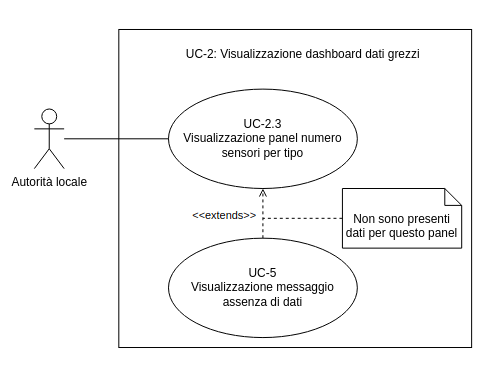
\includegraphics[width=0.75\textwidth]{analisi_dei_requisiti/UC-2.3.png}
	\captionof{figure}{UC-2.3: Visualizzazione \textit{panel} temperatura media}
\end{center}
\subsubsubsection{UC-2.4: Visualizzazione \textit{panel} temperatura massima}
\begin{itemize}
	\item \textbf{Attore principale}: Autorità locale;
	\item \textbf{Precondizioni}: 	\item \textbf{Postcondizioni}: L'autorità locale visualizza un \textit{panel} contenente la temperatura massima in un determinato periodo di tempo;
	      \begin{enumerate}
		      \item L'autorità locale ha effettuato l'accesso al sistema ed esso è in funzione;
		      \item Il sistema ha caricato la \href{https://7last.github.io/docs/rtb/documentazione-interna/glossario\#dashboard}{dashboard\textsubscript{G}} relativa ai \href{https://7last.github.io/docs/rtb/documentazione-interna/glossario\#dati-atmosferici}{dati atmosferici\textsubscript{G}};
	      \end{enumerate}
	\item \textbf{Postcondizioni}: L'autorità locale visualizza un \textit{panel} contenente la temperatura massima in un determinato periodo di tempo;
	\item \textbf{Scenario principale}:
	      \begin{enumerate}
		      \item L'autorità locale accede alla piattaforma;
		      \item Il sistema carica i dati relativi ai sensori interrogando il database;
		      \item L'autorità locale seleziona la visualizzazione della \href{https://7last.github.io/docs/rtb/documentazione-interna/glossario\#dashboard}{dashboard\textsubscript{G}} relativa ai \href{https://7last.github.io/docs/rtb/documentazione-interna/glossario\#dati-atmosferici}{dati atmosferici\textsubscript{G}}.
	      \end{enumerate}

	\item \href{https://7last.github.io/docs/rtb/documentazione-interna/glossario\#user-story}{\textbf{User story}\textsubscript{G}}: Come autorità locale desidero poter visualizzare la temperatura massima in un determinato periodo di tempo
	      in modo da poterne monitorare l'andamento.
\end{itemize}

\begin{center}
	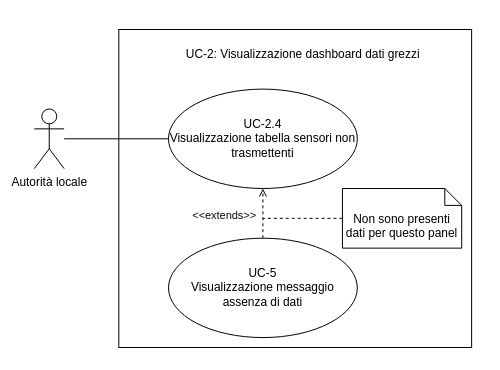
\includegraphics[width=0.75\textwidth]{analisi_dei_requisiti/UC-2.4.png}
	\captionof{figure}{UC-2.4: Visualizzazione \textit{panel} temperatura massima}
\end{center}
\subsubsubsection{UC-2.5: Visualizzazione \textit{panel} temperatura minima}
\begin{itemize}
	\item \textbf{Attore principale}: Autorità locale;
	\item \textbf{Precondizioni}:  	\item \textbf{Postcondizioni}: L'autorità locale visualizza un \textit{panel} contenente la temperatura minima in un determinato periodo di tempo;
	      \begin{enumerate}
		      \item L'autorità locale ha effettuato l'accesso al sistema ed esso è in funzione;
		      \item Il sistema ha caricato la \href{https://7last.github.io/docs/rtb/documentazione-interna/glossario\#dashboard}{dashboard\textsubscript{G}} relativa ai \href{https://7last.github.io/docs/rtb/documentazione-interna/glossario\#dati-atmosferici}{dati atmosferici\textsubscript{G}};
	      \end{enumerate}
	\item \textbf{Postcondizioni}: L'autorità locale visualizza un \textit{panel} contenente la temperatura minima in un determinato periodo di tempo;
	\item \textbf{Scenario principale}:
	      \begin{enumerate}
		      \item L'autorità locale accede alla piattaforma;
		      \item Il sistema carica i dati relativi ai sensori interrogando il database;
		      \item L'autorità locale seleziona la visualizzazione della \href{https://7last.github.io/docs/rtb/documentazione-interna/glossario\#dashboard}{dashboard\textsubscript{G}} relativa ai \href{https://7last.github.io/docs/rtb/documentazione-interna/glossario\#dati-atmosferici}{dati atmosferici\textsubscript{G}}.
	      \end{enumerate}
	\item \href{https://7last.github.io/docs/rtb/documentazione-interna/glossario\#user-story}{\textbf{User story}\textsubscript{G}}: Come autorità locale desidero poter visualizzare la temperatura minima in un determinato periodo di tempo
	      in modo da poterne monitorare l'andamento.
\end{itemize}

\begin{center}
	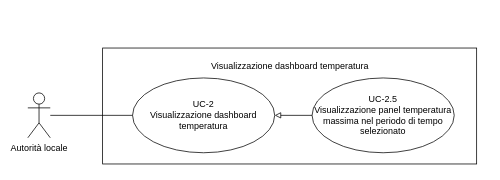
\includegraphics[width=0.75\textwidth]{analisi_dei_requisiti/UC-2.5.png}
	\captionof{figure}{UC-2.5: Visualizzazione \textit{panel} temperatura minima}
\end{center}

% umidità
\subsubsubsection{UC-2.6: Visualizzazione grafico time series per umidità}
\begin{itemize}
	\item \textbf{Attore principale}: Autorità locale;
	\item \textbf{Precondizioni}: 	\item \textbf{Postcondizioni}: L'autorità locale visualizza un grafico \href{https://7last.github.io/docs/rtb/documentazione-interna/glossario\#time-series}{time series\textsubscript{G}} contenente le misurazioni storiche
	      \begin{enumerate}
		      \item L'autorità locale ha effettuato l'accesso al sistema ed esso è in funzione;
		      \item Il sistema ha caricato la \href{https://7last.github.io/docs/rtb/documentazione-interna/glossario\#dashboard}{dashboard\textsubscript{G}} relativa ai \href{https://7last.github.io/docs/rtb/documentazione-interna/glossario\#dati-atmosferici}{dati atmosferici\textsubscript{G}};
	      \end{enumerate}
	\item \textbf{Postcondizioni}: L'autorità locale visualizza un grafico \href{https://7last.github.io/docs/rtb/documentazione-interna/glossario\#time-series}{time series\textsubscript{G}} contenente le misurazioni storiche
	      dell'umidità;
	\item \textbf{Scenario principale}:
	      \begin{enumerate}
		      \item L'autorità locale accede alla piattaforma;
		      \item Il sistema carica i dati relativi ai sensori interrogando il database;
		      \item L'autorità locale seleziona la visualizzazione della \href{https://7last.github.io/docs/rtb/documentazione-interna/glossario\#dashboard}{dashboard\textsubscript{G}} relativa ai \href{https://7last.github.io/docs/rtb/documentazione-interna/glossario\#dati-atmosferici}{dati atmosferici\textsubscript{G}}.
	      \end{enumerate}
	\item \href{https://7last.github.io/docs/rtb/documentazione-interna/glossario\#user-story}{\textbf{User story}\textsubscript{G}}: Come autorità locale desidero poter visualizzare un grafico \href{https://7last.github.io/docs/rtb/documentazione-interna/glossario\#time-series}{time series\textsubscript{G}} contenente le misurazioni storiche dell'umidità
	      per poter monitorarne l'andamento nel tempo e facilmente individuare eventuali anomalie.
\end{itemize}

\begin{center}
	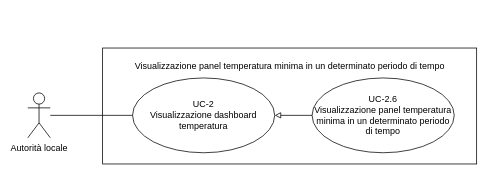
\includegraphics[width=0.75\textwidth]{analisi_dei_requisiti/UC-2.6.png}
	\captionof{figure}{UC-2.6: Visualizzazione grafico \href{https://7last.github.io/docs/rtb/documentazione-interna/glossario\#time-series}{time series\textsubscript{G}} per umidità}
\end{center}

\subsubsubsection{UC-2.7: Visualizzazione \textit{panel} umidità in tempo reale}
\begin{itemize}
	\item \textbf{Attore principale}: Autorità locale;
	\item \textbf{Precondizioni}:
	      \begin{enumerate}
		      \item L'autorità locale ha effettuato l'accesso al sistema ed esso è in funzione;
		      \item Il sistema ha caricato la \href{https://7last.github.io/docs/rtb/documentazione-interna/glossario\#dashboard}{dashboard\textsubscript{G}} relativa ai \href{https://7last.github.io/docs/rtb/documentazione-interna/glossario\#dati-atmosferici}{dati atmosferici\textsubscript{G}};
	      \end{enumerate}
	\item \textbf{Postcondizioni}: L'autorità locale visualizza un \textit{panel} contenente l'umidità in tempo reale;
	\item \textbf{Scenario principale}:
	      \begin{enumerate}
		      \item L'autorità locale accede alla piattaforma;
		      \item Il sistema carica i dati relativi ai sensori interrogando il database;
		      \item L'autorità locale seleziona la visualizzazione della \href{https://7last.github.io/docs/rtb/documentazione-interna/glossario\#dashboard}{dashboard\textsubscript{G}} relativa ai \href{https://7last.github.io/docs/rtb/documentazione-interna/glossario\#dati-atmosferici}{dati atmosferici\textsubscript{G}}.
	      \end{enumerate}
	\item \href{https://7last.github.io/docs/rtb/documentazione-interna/glossario\#user-story}{\textbf{User story}\textsubscript{G}}: Come autorità locale desidero poter visualizzare l'umidità in tempo reale per poter monitorare
	      l'andamento dell'umidità in tempo reale e prendere decisioni in base ad esso.
\end{itemize}

\begin{center}
	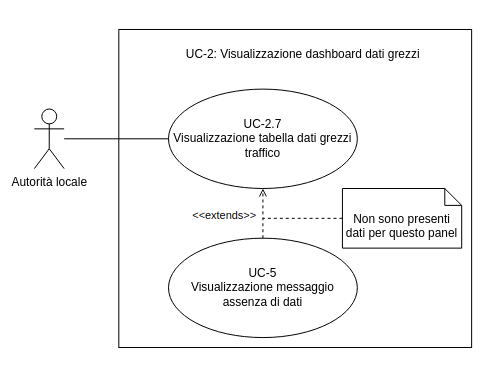
\includegraphics[width=0.75\textwidth]{analisi_dei_requisiti/UC-2.7.png}
	\captionof{figure}{UC-2.7: Visualizzazione \textit{panel} umidità in tempo reale}
\end{center}

\subsubsubsection{UC-2.8: Visualizzazione \textit{panel} umidità media}
\begin{itemize}
	\item \textbf{Attore principale}: Autorità locale;
	\item \textbf{Precondizioni}:
	      \begin{enumerate}
		      \item L'autorità locale ha effettuato l'accesso al sistema ed esso è in funzione;
		      \item Il sistema ha caricato la \href{https://7last.github.io/docs/rtb/documentazione-interna/glossario\#dashboard}{dashboard\textsubscript{G}} relativa ai \href{https://7last.github.io/docs/rtb/documentazione-interna/glossario\#dati-atmosferici}{dati atmosferici\textsubscript{G}};
	      \end{enumerate}
	\item \textbf{Postcondizioni}: L'autorità locale visualizza un \textit{panel} contenente l'umidità media in un determinato periodo di tempo;
	\item \textbf{Scenario principale}:
	      \begin{enumerate}
		      \item L'autorità locale accede alla piattaforma;
		      \item Il sistema carica i dati relativi ai sensori interrogando il database;
		      \item L'autorità locale seleziona la visualizzazione della \href{https://7last.github.io/docs/rtb/documentazione-interna/glossario\#dashboard}{dashboard\textsubscript{G}} relativa ai \href{https://7last.github.io/docs/rtb/documentazione-interna/glossario\#dati-atmosferici}{dati atmosferici\textsubscript{G}}.
	      \end{enumerate}
	\item \href{https://7last.github.io/docs/rtb/documentazione-interna/glossario\#user-story}{\textbf{User story}\textsubscript{G}}: Come autorità locale desidero poter visualizzare l'umidità media in un determinato periodo di tempo
	      in modo da poterne monitorare l'andamento.
\end{itemize}

\begin{center}
	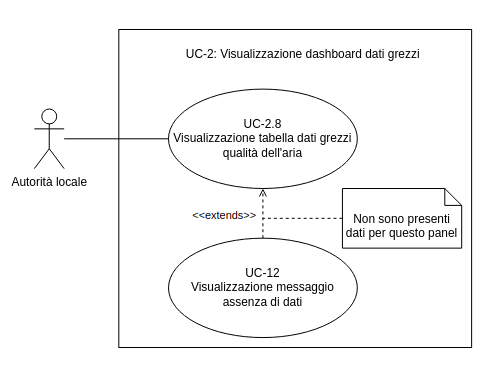
\includegraphics[width=0.75\textwidth]{analisi_dei_requisiti/UC-2.8.png}
	\captionof{figure}{UC-2.8: Visualizzazione \textit{panel} umidità media}
\end{center}

\subsubsubsection{UC-2.9: Visualizzazione \textit{panel} umidità massima}
\begin{itemize}
	\item \textbf{Attore principale}: Autorità locale;
	\item \textbf{Precondizioni}:
	      \begin{enumerate}
		      \item L'autorità locale ha effettuato l'accesso al sistema ed esso è in funzione;
		      \item Il sistema ha caricato la \href{https://7last.github.io/docs/rtb/documentazione-interna/glossario\#dashboard}{dashboard\textsubscript{G}} relativa ai \href{https://7last.github.io/docs/rtb/documentazione-interna/glossario\#dati-atmosferici}{dati atmosferici\textsubscript{G}};
	      \end{enumerate}
	\item \textbf{Postcondizioni}: L'autorità locale visualizza un \textit{panel} contenente l'umidità massima in un determinato periodo di tempo;
	\item \textbf{Scenario principale}:
	      \begin{enumerate}
		      \item L'autorità locale accede alla piattaforma;
		      \item Il sistema carica i dati relativi ai sensori interrogando il database;
		      \item L'autorità locale seleziona la visualizzazione della \href{https://7last.github.io/docs/rtb/documentazione-interna/glossario\#dashboard}{dashboard\textsubscript{G}} relativa ai \href{https://7last.github.io/docs/rtb/documentazione-interna/glossario\#dati-atmosferici}{dati atmosferici\textsubscript{G}}.
	      \end{enumerate}
	\item \href{https://7last.github.io/docs/rtb/documentazione-interna/glossario\#user-story}{\textbf{User story}\textsubscript{G}}: Come autorità locale desidero poter visualizzare l'umidità massima in un determinato periodo di tempo
	      in modo da poterne monitorare l'andamento.
\end{itemize}

\begin{center}
	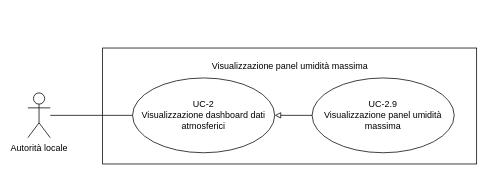
\includegraphics[width=0.75\textwidth]{analisi_dei_requisiti/UC-2.9.png}
	\captionof{figure}{UC-2.9: Visualizzazione \textit{panel} umidità massima}
\end{center}

\subsubsubsection{UC-2.10: Visualizzazione \textit{panel} umidità minima}
\begin{itemize}
	\item \textbf{Attore principale}: Autorità locale;
	\item \textbf{Precondizioni}:
	      \begin{enumerate}
		      \item L'autorità locale ha effettuato l'accesso al sistema ed esso è in funzione;
		      \item Il sistema ha caricato la \href{https://7last.github.io/docs/rtb/documentazione-interna/glossario\#dashboard}{dashboard\textsubscript{G}} relativa ai \href{https://7last.github.io/docs/rtb/documentazione-interna/glossario\#dati-atmosferici}{dati atmosferici\textsubscript{G}};
	      \end{enumerate}
	\item \textbf{Postcondizioni}: L'autorità locale visualizza un \textit{panel} contenente l'umidità minima in un determinato periodo di tempo;
	\item \textbf{Scenario principale}:
	      \begin{enumerate}
		      \item L'autorità locale accede alla piattaforma;
		      \item Il sistema carica i dati relativi ai sensori interrogando il database;
		      \item L'autorità locale seleziona la visualizzazione della \href{https://7last.github.io/docs/rtb/documentazione-interna/glossario\#dashboard}{dashboard\textsubscript{G}} relativa ai \href{https://7last.github.io/docs/rtb/documentazione-interna/glossario\#dati-atmosferici}{dati atmosferici\textsubscript{G}}.
	      \end{enumerate}
	\item \href{https://7last.github.io/docs/rtb/documentazione-interna/glossario\#user-story}{\textbf{User story}\textsubscript{G}}: Come autorità locale desidero poter visualizzare l'umidità minima in un determinato periodo di tempo
	      in modo da poterne monitorare l'andamento.
\end{itemize}

\begin{center}
	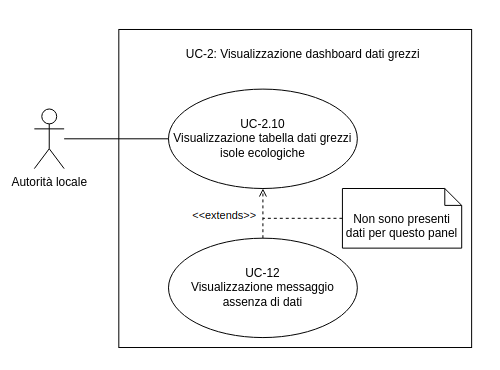
\includegraphics[width=0.75\textwidth]{analisi_dei_requisiti/UC-2.10.png}
	\captionof{figure}{UC-2.10: Visualizzazione \textit{panel} umidità minima}
\end{center}

% pressione
\subsubsubsection{UC-2.11: Visualizzazione grafico time series per pressione}
\begin{itemize}
	\item \textbf{Attore principale}: Autorità locale;
	\item \textbf{Precondizioni}:
	      \begin{enumerate}
		      \item L'autorità locale ha effettuato l'accesso al sistema ed esso è in funzione;
		      \item Il sistema ha caricato la \href{https://7last.github.io/docs/rtb/documentazione-interna/glossario\#dashboard}{dashboard\textsubscript{G}} relativa ai \href{https://7last.github.io/docs/rtb/documentazione-interna/glossario\#dati-atmosferici}{dati atmosferici\textsubscript{G}};
	      \end{enumerate}
	\item \textbf{Postcondizioni}: L'autorità locale visualizza un grafico \href{https://7last.github.io/docs/rtb/documentazione-interna/glossario\#time-series}{time series\textsubscript{G}} contenente le misurazioni storiche
	\item \textbf{Scenario principale}:
	      \begin{enumerate}
		      \item L'autorità locale accede alla piattaforma;
		      \item Il sistema carica i dati relativi ai sensori interrogando il database;
		      \item L'autorità locale seleziona la visualizzazione della \href{https://7last.github.io/docs/rtb/documentazione-interna/glossario\#dashboard}{dashboard\textsubscript{G}} relativa ai \href{https://7last.github.io/docs/rtb/documentazione-interna/glossario\#dati-atmosferici}{dati atmosferici\textsubscript{G}}.
	      \end{enumerate}
	\item \href{https://7last.github.io/docs/rtb/documentazione-interna/glossario\#user-story}{\textbf{User story}\textsubscript{G}}: Come autorità locale desidero poter visualizzare un grafico \href{https://7last.github.io/docs/rtb/documentazione-interna/glossario\#time-series}{time series\textsubscript{G}} contenente le misurazioni storiche della pressione
	      per poter monitorarne l'andamento nel tempo e facilmente individuare eventuali anomalie.
\end{itemize}

\begin{center}
	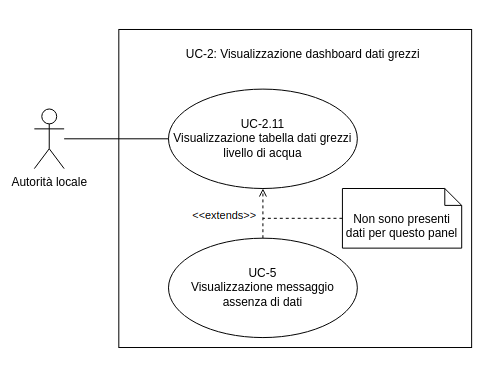
\includegraphics[width=0.75\textwidth]{analisi_dei_requisiti/UC-2.11.png}
	\captionof{figure}{UC-2.11: Visualizzazione grafico \href{https://7last.github.io/docs/rtb/documentazione-interna/glossario\#time-series}{time series\textsubscript{G}} per pressione}
\end{center}
\subsubsubsection{UC-2.12: Visualizzazione \textit{panel} pressione in tempo reale}
\begin{itemize}
	\item \textbf{Attore principale}: Autorità locale;
	\item \textbf{Precondizioni}:
	      \begin{enumerate}
		      \item L'autorità locale ha effettuato l'accesso al sistema ed esso è in funzione;
		      \item Il sistema ha caricato la \href{https://7last.github.io/docs/rtb/documentazione-interna/glossario\#dashboard}{dashboard\textsubscript{G}} relativa ai \href{https://7last.github.io/docs/rtb/documentazione-interna/glossario\#dati-atmosferici}{dati atmosferici\textsubscript{G}};
	      \end{enumerate}
	\item \textbf{Postcondizioni}: L'autorità locale visualizza un \textit{panel} contenente la pressione in tempo reale;
	\item \textbf{Scenario principale}:
	      \begin{enumerate}
		      \item L'autorità locale accede alla piattaforma;
		      \item Il sistema carica i dati relativi ai sensori interrogando il database;
	      \end{enumerate}
	\item \href{https://7last.github.io/docs/rtb/documentazione-interna/glossario\#user-story}{\textbf{User story}\textsubscript{G}}: Come autorità locale desidero poter visualizzare la pressione in tempo reale per poter monitorare
	      l'andamento della pressione in tempo reale e prendere decisioni in base ad esso.
\end{itemize}

\begin{center}
	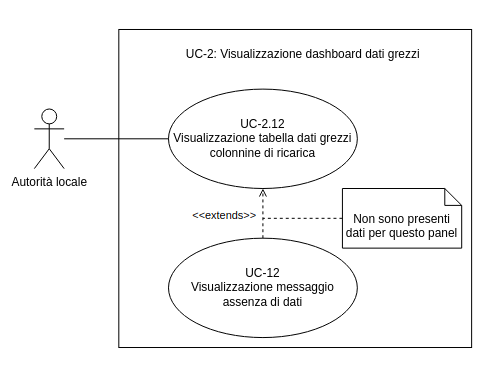
\includegraphics[width=0.75\textwidth]{analisi_dei_requisiti/UC-2.12.png}
	\captionof{figure}{UC-2.12: Visualizzazione \textit{panel} pressione in tempo reale}
\end{center}
\subsubsubsection{UC-2.13: Visualizzazione \textit{panel} pressione media}
\begin{itemize}
	\item \textbf{Attore principale}: Autorità locale;
	\item \textbf{Precondizioni}:
	      \begin{enumerate}
		      \item L'autorità locale ha effettuato l'accesso al sistema ed esso è in funzione;
		      \item Il sistema ha caricato la \href{https://7last.github.io/docs/rtb/documentazione-interna/glossario\#dashboard}{dashboard\textsubscript{G}} relativa ai \href{https://7last.github.io/docs/rtb/documentazione-interna/glossario\#dati-atmosferici}{dati atmosferici\textsubscript{G}};
	      \end{enumerate}

	\item \textbf{Postcondizioni}: L'autorità locale visualizza un \textit{panel} contenente la pressione media in un determinato periodo di tempo;
	\item \textbf{Scenario principale}:
	      \begin{enumerate}
		      \item L'autorità locale accede alla piattaforma;
		      \item Il sistema carica i dati relativi ai sensori interrogando il database;
		      \item L'autorità locale seleziona la visualizzazione della \href{https://7last.github.io/docs/rtb/documentazione-interna/glossario\#dashboard}{dashboard\textsubscript{G}} relativa ai \href{https://7last.github.io/docs/rtb/documentazione-interna/glossario\#dati-atmosferici}{dati atmosferici\textsubscript{G}}.
	      \end{enumerate}
	\item \href{https://7last.github.io/docs/rtb/documentazione-interna/glossario\#user-story}{\textbf{User story}\textsubscript{G}}: Come autorità locale desidero poter visualizzare la pressione media in un determinato periodo di tempo
	      in modo da poterne monitorare l'andamento.
\end{itemize}

\begin{center}
	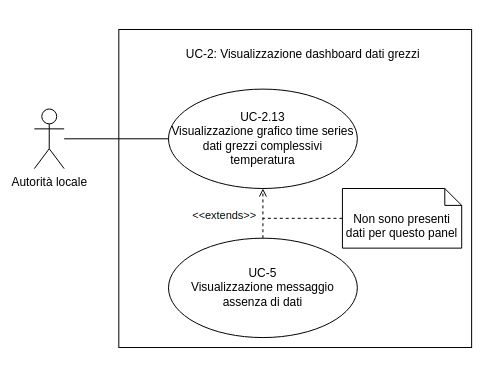
\includegraphics[width=0.75\textwidth]{analisi_dei_requisiti/UC-2.13.png}
	\captionof{figure}{UC-2.13: Visualizzazione \textit{panel} pressione media}
\end{center}
\subsubsubsection{UC-2.14: Visualizzazione \textit{panel} pressione massima}
\begin{itemize}
	\item \textbf{Attore principale}: Autorità locale;
	\item \textbf{Precondizioni}:
	      \begin{enumerate}
		      \item L'autorità locale ha effettuato l'accesso al sistema ed esso è in funzione;
		      \item Il sistema ha caricato la \href{https://7last.github.io/docs/rtb/documentazione-interna/glossario\#dashboard}{dashboard\textsubscript{G}} relativa ai \href{https://7last.github.io/docs/rtb/documentazione-interna/glossario\#dati-atmosferici}{dati atmosferici\textsubscript{G}};
	      \end{enumerate}
	\item \textbf{Postcondizioni}: L'autorità locale visualizza un \textit{panel} contenente la pressione massima in un determinato periodo di tempo;
	\item \textbf{Scenario principale}:
	      \begin{enumerate}
		      \item L'autorità locale accede alla piattaforma;
		      \item Il sistema carica i dati relativi ai sensori interrogando il database;
		      \item L'autorità locale seleziona la visualizzazione della \href{https://7last.github.io/docs/rtb/documentazione-interna/glossario\#dashboard}{dashboard\textsubscript{G}} relativa ai \href{https://7last.github.io/docs/rtb/documentazione-interna/glossario\#dati-atmosferici}{dati atmosferici\textsubscript{G}}.
	      \end{enumerate}
	\item \href{https://7last.github.io/docs/rtb/documentazione-interna/glossario\#user-story}{\textbf{User story}\textsubscript{G}}: Come autorità locale desidero poter visualizzare la pressione massima in un determinato periodo di tempo
	      in modo da poterne monitorare l'andamento.
\end{itemize}

\begin{center}
	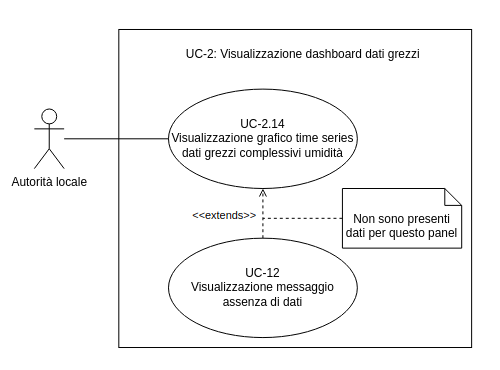
\includegraphics[width=0.75\textwidth]{analisi_dei_requisiti/UC-2.14.png}
	\captionof{figure}{UC-2.14: Visualizzazione \textit{panel} pressione massima}
\end{center}
\subsubsubsection{UC-2.15: Visualizzazione \textit{panel} pressione minima}
\begin{itemize}
	\item \textbf{Attore principale}: Autorità locale;
	\item \textbf{Precondizioni}:
	      \begin{enumerate}
		      \item L'autorità locale ha effettuato l'accesso al sistema ed esso è in funzione;
		      \item Il sistema ha caricato la \href{https://7last.github.io/docs/rtb/documentazione-interna/glossario\#dashboard}{dashboard\textsubscript{G}} relativa ai \href{https://7last.github.io/docs/rtb/documentazione-interna/glossario\#dati-atmosferici}{dati atmosferici\textsubscript{G}};
	      \end{enumerate}
	\item \textbf{Postcondizioni}: L'autorità locale visualizza un \textit{panel} contenente la pressione minima in un determinato periodo di tempo;
	\item \textbf{Scenario principale}:
	      \begin{enumerate}
		      \item L'autorità locale accede alla piattaforma;
		      \item Il sistema carica i dati relativi ai sensori interrogando il database;
		      \item L'autorità locale seleziona la visualizzazione della \href{https://7last.github.io/docs/rtb/documentazione-interna/glossario\#dashboard}{dashboard\textsubscript{G}} relativa ai \href{https://7last.github.io/docs/rtb/documentazione-interna/glossario\#dati-atmosferici}{dati atmosferici\textsubscript{G}}.
	      \end{enumerate}
	\item \href{https://7last.github.io/docs/rtb/documentazione-interna/glossario\#user-story}{\textbf{User story}\textsubscript{G}}: Come autorità locale desidero poter visualizzare la pressione minima in un determinato periodo di tempo
	      in modo da poterne monitorare l'andamento.
\end{itemize}

\begin{center}
	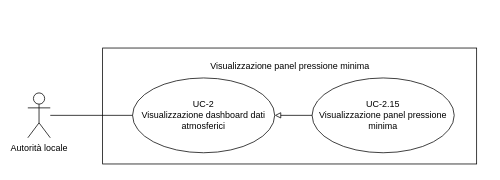
\includegraphics[width=0.75\textwidth]{analisi_dei_requisiti/UC-2.15.png}
	\captionof{figure}{UC-2.15: Visualizzazione \textit{panel} pressione minima}
\end{center}

% precipitazioni
\subsubsubsection{UC-2.16: Visualizzazione grafico time series per quantità di precipitazioni}
\begin{itemize}
	\item \textbf{Attore principale}: Autorità locale;
	\item \textbf{Precondizioni}:
	      \begin{enumerate}
		      \item L'autorità locale ha effettuato l'accesso al sistema ed esso è in funzione;
		      \item Il sistema ha caricato la \href{https://7last.github.io/docs/rtb/documentazione-interna/glossario\#dashboard}{dashboard\textsubscript{G}} relativa ai \href{https://7last.github.io/docs/rtb/documentazione-interna/glossario\#dati-atmosferici}{dati atmosferici\textsubscript{G}};
	      \end{enumerate}

	\item \textbf{Postcondizioni}: L'autorità locale visualizza un grafico \href{https://7last.github.io/docs/rtb/documentazione-interna/glossario\#time-series}{time series\textsubscript{G}} contenente le misurazioni storiche
	      della quantità di precipitazioni;

	\item \textbf{Scenario principale}:
	      \begin{enumerate}
		      \item L'autorità locale accede alla piattaforma;
		      \item Il sistema carica i dati relativi ai sensori interrogando il database;
		      \item L'autorità locale seleziona la visualizzazione della \href{https://7last.github.io/docs/rtb/documentazione-interna/glossario\#dashboard}{dashboard\textsubscript{G}} relativa ai \href{https://7last.github.io/docs/rtb/documentazione-interna/glossario\#dati-atmosferici}{dati atmosferici\textsubscript{G}}.
	      \end{enumerate}
	\item \href{https://7last.github.io/docs/rtb/documentazione-interna/glossario\#user-story}{\textbf{User story}\textsubscript{G}}: Come autorità locale desidero poter visualizzare un grafico \href{https://7last.github.io/docs/rtb/documentazione-interna/glossario\#time-series}{time series\textsubscript{G}} contenente le misurazioni storiche della quantità di precipitazioni
	      per poter monitorarne l'andamento nel tempo e facilmente individuare eventuali anomalie.

\end{itemize}

\begin{center}
	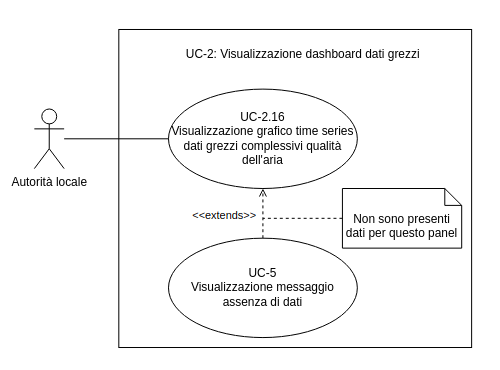
\includegraphics[width=0.75\textwidth]{analisi_dei_requisiti/UC-2.16.png}
	\captionof{figure}{UC-2.16: Visualizzazione grafico \href{https://7last.github.io/docs/rtb/documentazione-interna/glossario\#time-series}{time series\textsubscript{G}} per precipitazioni}
\end{center}

\subsubsubsection{UC-2.17: Visualizzazione \textit{panel} quantità di precipitazioni in tempo reale}
\begin{itemize}
	\item \textbf{Attore principale}: Autorità locale;
	\item \textbf{Precondizioni}:
	      \begin{enumerate}
		      \item L'autorità locale ha effettuato l'accesso al sistema ed esso è in funzione;
		      \item Il sistema ha caricato la \href{https://7last.github.io/docs/rtb/documentazione-interna/glossario\#dashboard}{dashboard\textsubscript{G}} relativa ai \href{https://7last.github.io/docs/rtb/documentazione-interna/glossario\#dati-atmosferici}{dati atmosferici\textsubscript{G}};
	      \end{enumerate}

	\item \textbf{Postcondizioni}: L'autorità locale visualizza un \textit{panel} contenente la quantità di precipitazioni in tempo reale;
	\item \textbf{Scenario principale}:
	      \begin{enumerate}
		      \item L'autorità locale accede alla piattaforma;
		      \item Il sistema carica i dati relativi ai sensori interrogando il database;
		      \item L'autorità locale seleziona la visualizzazione della \href{https://7last.github.io/docs/rtb/documentazione-interna/glossario\#dashboard}{dashboard\textsubscript{G}} relativa ai \href{https://7last.github.io/docs/rtb/documentazione-interna/glossario\#dati-atmosferici}{dati atmosferici\textsubscript{G}}.
	      \end{enumerate}
	\item \href{https://7last.github.io/docs/rtb/documentazione-interna/glossario\#user-story}{\textbf{User story}\textsubscript{G}}: Come autorità locale desidero poter visualizzare la quantità di precipitazioni in tempo reale per poter monitorare
	      l'andamento delle precipitazioni in tempo reale e prendere decisioni in base ad esso.
\end{itemize}

\begin{center}
	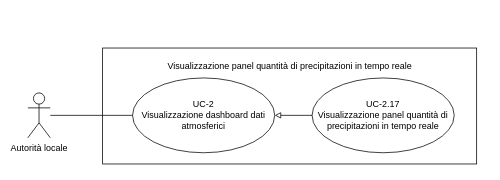
\includegraphics[width=0.75\textwidth]{analisi_dei_requisiti/UC-2.17.png}
	\captionof{figure}{UC-2.17: Visualizzazione \textit{panel} quantità di precipitazioni in tempo reale}
\end{center}

\subsubsubsection{UC-2.18: Visualizzazione \textit{panel} quantità totale di precipitazioni}
\begin{itemize}
	\item \textbf{Attore principale}: Autorità locale;
	\item \textbf{Precondizioni}:
	      \begin{enumerate}
		      \item L'autorità locale ha effettuato l'accesso al sistema ed esso è in funzione;
		      \item Il sistema ha caricato la \href{https://7last.github.io/docs/rtb/documentazione-interna/glossario\#dashboard}{dashboard\textsubscript{G}} relativa ai \href{https://7last.github.io/docs/rtb/documentazione-interna/glossario\#dati-atmosferici}{dati atmosferici\textsubscript{G}};
	      \end{enumerate}
	\item \textbf{Postcondizioni}: L'autorità locale visualizza un \textit{panel} contenente la quantità totale di precipitazioni in un dato periodo di tempo
	\item \textbf{Scenario principale}:
	      \begin{enumerate}
		      \item L'autorità locale accede alla piattaforma;
		      \item Il sistema carica i dati relativi ai sensori interrogando il database;
		      \item L'autorità locale seleziona la visualizzazione della \href{https://7last.github.io/docs/rtb/documentazione-interna/glossario\#dashboard}{dashboard\textsubscript{G}} relativa ai \href{https://7last.github.io/docs/rtb/documentazione-interna/glossario\#dati-atmosferici}{dati atmosferici\textsubscript{G}}.
	      \end{enumerate}
	\item \href{https://7last.github.io/docs/rtb/documentazione-interna/glossario\#user-story}{\textbf{User story}\textsubscript{G}}: Come autorità locale desidero poter visualizzare la quantità totale di precipitazioni in un dato periodo di tempo.
\end{itemize}

\begin{center}
	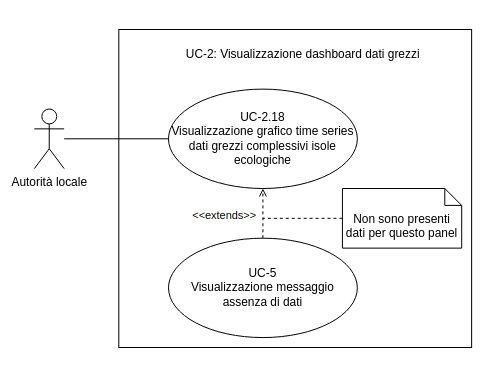
\includegraphics[width=0.75\textwidth]{analisi_dei_requisiti/UC-2.18.png}
	\captionof{figure}{UC-2.18: Visualizzazione \textit{panel} quantità totale di precipitazioni}
\end{center}

\subsubsubsection{UC-2.19: Visualizzazione \textit{panel} quantità media di precipitazioni}
\begin{itemize}
	\item \textbf{Attore principale}: Autorità locale;
	\item \textbf{Precondizioni}:
	      \begin{enumerate}
		      \item L'autorità locale ha effettuato l'accesso al sistema ed esso è in funzione;
		      \item Il sistema ha caricato la \href{https://7last.github.io/docs/rtb/documentazione-interna/glossario\#dashboard}{dashboard\textsubscript{G}} relativa ai \href{https://7last.github.io/docs/rtb/documentazione-interna/glossario\#dati-atmosferici}{dati atmosferici\textsubscript{G}};
	      \end{enumerate}
	\item \textbf{Postcondizioni}: L'autorità locale visualizza un \textit{panel} contenente la quantità media di precipitazioni in
	      un dato periodo di tempo;
	\item \textbf{Scenario principale}:
	      \begin{enumerate}
		      \item L'autorità locale accede alla piattaforma;
		      \item Il sistema carica i dati relativi ai sensori interrogando il database;
		      \item L'autorità locale seleziona la visualizzazione della \href{https://7last.github.io/docs/rtb/documentazione-interna/glossario\#dashboard}{dashboard\textsubscript{G}} relativa ai \href{https://7last.github.io/docs/rtb/documentazione-interna/glossario\#dati-atmosferici}{dati atmosferici\textsubscript{G}}.
	      \end{enumerate}
	\item \href{https://7last.github.io/docs/rtb/documentazione-interna/glossario\#user-story}{\textbf{User story}\textsubscript{G}}: Come autorità locale desidero poter visualizzare la quantità media di precipitazioni in un dato periodo di tempo.
\end{itemize}

\begin{center}
	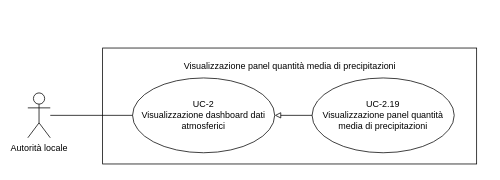
\includegraphics[width=0.75\textwidth]{analisi_dei_requisiti/UC-2.19.png}
	\captionof{figure}{UC-2.19: Visualizzazione \textit{panel} quantità media di precipitazioni}
\end{center}

% polveri sottili
\subsubsubsection{UC-2.20: Visualizzazione grafico time series per polveri sottili nell'aria}
\begin{itemize}
	\item \textbf{Attore principale}: Autorità locale;
	\item \textbf{Precondizioni}:
	      \begin{enumerate}
		      \item L'autorità locale ha effettuato l'accesso al sistema ed esso è in funzione;
		      \item Il sistema ha caricato la \href{https://7last.github.io/docs/rtb/documentazione-interna/glossario\#dashboard}{dashboard\textsubscript{G}} relativa ai \href{https://7last.github.io/docs/rtb/documentazione-interna/glossario\#dati-atmosferici}{dati atmosferici\textsubscript{G}};
	      \end{enumerate}
	\item \textbf{Postcondizioni}: L'autorità locale visualizza un grafico \href{https://7last.github.io/docs/rtb/documentazione-interna/glossario\#time-series}{time series\textsubscript{G}} contenente le misurazioni storiche
	      delle polveri sottili nell'aria;
	\item \textbf{Scenario principale}:
	      \begin{enumerate}
		      \item L'autorità locale accede alla piattaforma;
		      \item Il sistema carica i dati relativi ai sensori interrogando il database;
		      \item L'autorità locale seleziona la visualizzazione della \href{https://7last.github.io/docs/rtb/documentazione-interna/glossario\#dashboard}{dashboard\textsubscript{G}} relativa ai \href{https://7last.github.io/docs/rtb/documentazione-interna/glossario\#dati-atmosferici}{dati atmosferici\textsubscript{G}}.
	      \end{enumerate}
	\item \href{https://7last.github.io/docs/rtb/documentazione-interna/glossario\#user-story}{\textbf{User story}\textsubscript{G}}: Come autorità locale desidero poter visualizzare un grafico \href{https://7last.github.io/docs/rtb/documentazione-interna/glossario\#time-series}{time series\textsubscript{G}} contenente le misurazioni storiche delle polveri sottili nell'aria
	      per poter monitorarne l'andamento nel tempo e facilmente individuare eventuali anomalie.
\end{itemize}

\begin{center}
	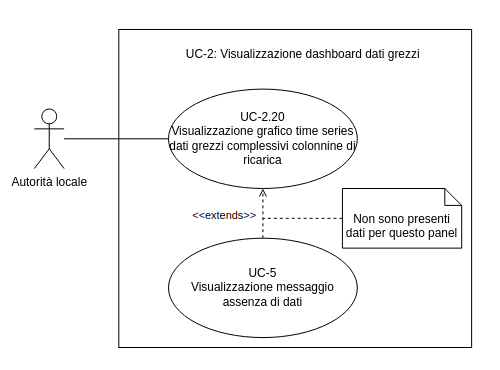
\includegraphics[width=0.75\textwidth]{analisi_dei_requisiti/UC-2.20.png}
	\captionof{figure}{UC-2.20: Visualizzazione grafico \href{https://7last.github.io/docs/rtb/documentazione-interna/glossario\#time-series}{time series\textsubscript{G}} per polveri sottili nell'aria}
\end{center}

\subsubsubsection{UC-2.21: Visualizzazione \textit{panel} polveri sottili nell'aria in tempo reale}
\begin{itemize}
	\item \textbf{Attore principale}: Autorità locale;
	\item \textbf{Precondizioni}:
	      \begin{enumerate}
		      \item L'autorità locale ha effettuato l'accesso al sistema ed esso è in funzione;
		      \item Il sistema ha caricato la \href{https://7last.github.io/docs/rtb/documentazione-interna/glossario\#dashboard}{dashboard\textsubscript{G}} relativa ai \href{https://7last.github.io/docs/rtb/documentazione-interna/glossario\#dati-atmosferici}{dati atmosferici\textsubscript{G}};
	      \end{enumerate}
	\item \textbf{Postcondizioni}: L'autorità locale visualizza un \textit{panel} contenente la quantità di polveri sottili nell'aria in tempo reale;
	\item \textbf{Scenario principale}:
	      \begin{enumerate}
		      \item L'autorità locale accede alla piattaforma;
		      \item Il sistema carica i dati relativi ai sensori interrogando il database;
		      \item L'autorità locale seleziona la visualizzazione della \href{https://7last.github.io/docs/rtb/documentazione-interna/glossario\#dashboard}{dashboard\textsubscript{G}} relativa ai \href{https://7last.github.io/docs/rtb/documentazione-interna/glossario\#dati-atmosferici}{dati atmosferici\textsubscript{G}}.
	      \end{enumerate}
	\item \href{https://7last.github.io/docs/rtb/documentazione-interna/glossario\#user-story}{\textbf{User story}\textsubscript{G}}: Come autorità locale desidero poter visualizzare la quantità di polveri sottili nell'aria in tempo reale
	      l'andamento delle precipitazioni in tempo reale e prendere decisioni in base ad esso.
\end{itemize}

\begin{center}
	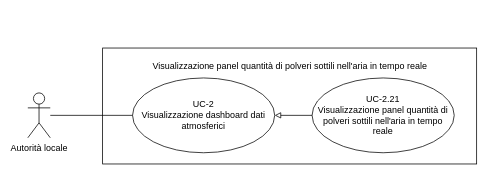
\includegraphics[width=0.75\textwidth]{analisi_dei_requisiti/UC-2.21.png}
	\captionof{figure}{UC-2.21: Visualizzazione \textit{panel} polveri sottili nell'aria in tempo reale}
\end{center}

\subsubsubsection{UC-2.22: Visualizzazione \textit{panel} giorno con maggiore concentrazione di polveri sottili}
\begin{itemize}
	\item \textbf{Attore principale}: Autorità locale;
	\item \textbf{Precondizioni}:
	      \begin{enumerate}
		      \item L'autorità locale ha effettuato l'accesso al sistema ed esso è in funzione;
		      \item Il sistema ha caricato la \href{https://7last.github.io/docs/rtb/documentazione-interna/glossario\#dashboard}{dashboard\textsubscript{G}} relativa ai \href{https://7last.github.io/docs/rtb/documentazione-interna/glossario\#dati-atmosferici}{dati atmosferici\textsubscript{G}};
	      \end{enumerate}
	\item \textbf{Postcondizioni}: L'autorità locale visualizza un \textit{panel} contenente il giorno con la maggiore concentrazione di polveri sottili
	      in un dato periodo di tempo;
	\item \textbf{Scenario principale}:
	      \begin{enumerate}
		      \item L'autorità locale accede alla piattaforma;
		      \item Il sistema carica i dati relativi ai sensori interrogando il database;
		      \item L'autorità locale seleziona la visualizzazione della \href{https://7last.github.io/docs/rtb/documentazione-interna/glossario\#dashboard}{dashboard\textsubscript{G}} relativa ai \href{https://7last.github.io/docs/rtb/documentazione-interna/glossario\#dati-atmosferici}{dati atmosferici\textsubscript{G}}.
	      \end{enumerate}
	\item \href{https://7last.github.io/docs/rtb/documentazione-interna/glossario\#user-story}{\textbf{User story}\textsubscript{G}}: Come autorità locale desidero poter visualizzare il giorno con la maggiore concentrazione di polveri sottili
	      in un dato periodo di tempo per poterne monitorare l'andamento e prendere decisioni in base ad esso.
\end{itemize}

\begin{center}
	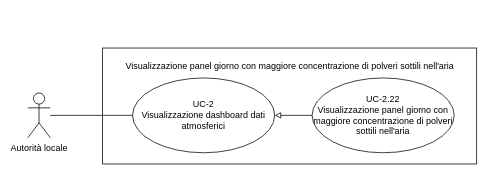
\includegraphics[width=0.75\textwidth]{analisi_dei_requisiti/UC-2.22.png}
	\captionof{figure}{UC-2.22: Visualizzazione \textit{panel} giorno con maggiore concentrazione di polveri sottili}
\end{center}

\subsubsubsection{UC-2.23: Visualizzazione \textit{panel} giorno con minore concentrazione di polveri sottili}
\begin{itemize}
	\item \textbf{Attore principale}: Autorità locale;
	\item \textbf{Precondizioni}:
	      \begin{enumerate}
		      \item L'autorità locale ha effettuato l'accesso al sistema ed esso è in funzione;
		      \item Il sistema ha caricato la \href{https://7last.github.io/docs/rtb/documentazione-interna/glossario\#dashboard}{dashboard\textsubscript{G}} relativa ai \href{https://7last.github.io/docs/rtb/documentazione-interna/glossario\#dati-atmosferici}{dati atmosferici\textsubscript{G}};
	      \end{enumerate}
	\item \textbf{Postcondizioni}: L'autorità locale visualizza un \textit{panel} contenente il giorno con la minore concentrazione di polveri sottili
	      in un dato periodo di tempo;
	\item \textbf{Scenario principale}:
	      \begin{enumerate}
		      \item L'autorità locale accede alla piattaforma;
		      \item Il sistema carica i dati relativi ai sensori interrogando il database;
		      \item L'autorità locale seleziona la visualizzazione della \href{https://7last.github.io/docs/rtb/documentazione-interna/glossario\#dashboard}{dashboard\textsubscript{G}} relativa ai \href{https://7last.github.io/docs/rtb/documentazione-interna/glossario\#dati-atmosferici}{dati atmosferici\textsubscript{G}}.
	      \end{enumerate}
	\item \href{https://7last.github.io/docs/rtb/documentazione-interna/glossario\#user-story}{\textbf{User story}\textsubscript{G}}: Come autorità locale desidero poter visualizzare il giorno con la minore concentrazione di polveri sottili
	      in un dato periodo di tempo per poterne monitorare l'andamento e prendere decisioni in base ad esso.
\end{itemize}


\begin{center}
	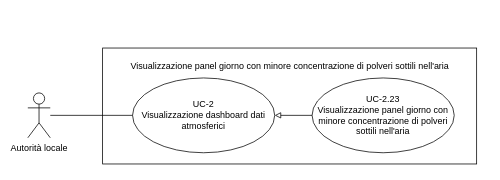
\includegraphics[width=0.75\textwidth]{analisi_dei_requisiti/UC-2.23.png}
	\captionof{figure}{UC-2.23: Visualizzazione \textit{panel} giorno con minore concentrazione di polveri sottili}
\end{center}

\subsubsubsection{UC-2.24: Visualizzazione \textit{panel} media di polveri sottili nell'aria}
\begin{itemize}
	\item \textbf{Attore principale}: Autorità locale;
	\item \textbf{Precondizioni}:
	      \begin{enumerate}
		      \item L'autorità locale ha effettuato l'accesso al sistema ed esso è in funzione;
		      \item Il sistema ha caricato la \href{https://7last.github.io/docs/rtb/documentazione-interna/glossario\#dashboard}{dashboard\textsubscript{G}} relativa ai \href{https://7last.github.io/docs/rtb/documentazione-interna/glossario\#dati-atmosferici}{dati atmosferici\textsubscript{G}};
	      \end{enumerate}
	\item \textbf{Postcondizioni}: L'autorità locale visualizza un \textit{panel} contenente la quantità media di polveri sottili nell'aria
	      in un dato periodo di tempo;
	\item \textbf{Scenario principale}:
	      \begin{enumerate}
		      \item L'autorità locale accede alla piattaforma;
		      \item Il sistema carica i dati relativi ai sensori interrogando il database;
		      \item L'autorità locale seleziona la visualizzazione della \href{https://7last.github.io/docs/rtb/documentazione-interna/glossario\#dashboard}{dashboard\textsubscript{G}} relativa ai \href{https://7last.github.io/docs/rtb/documentazione-interna/glossario\#dati-atmosferici}{dati atmosferici\textsubscript{G}}.
	      \end{enumerate}
	\item \href{https://7last.github.io/docs/rtb/documentazione-interna/glossario\#user-story}{\textbf{User story}\textsubscript{G}}: Come autorità locale desidero poter visualizzare un \textit{panel} contenente la quantità media di polveri sottili nell'aria
	      in un dato periodo di tempo per poterne monitorare l'andamento.
\end{itemize}

\begin{center}
	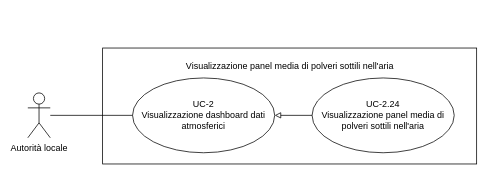
\includegraphics[width=0.75\textwidth]{analisi_dei_requisiti/UC-2.24.png}
	\captionof{figure}{UC-2.24: Visualizzazione \textit{panel} media di polveri sottili nell'aria}
\end{center}

\subsubsection{UC-3: Visualizzazione dashboard dati urbani}
\begin{itemize}
	\item \textbf{Attore principale}: Autorità locale;
	\item \textbf{Precondizioni}:
	      \begin{enumerate}
		      \item L'autorità locale ha effettuato l'accesso al sistema ed esso è in funzione;
		      \item Il sistema ha caricato la \href{https://7last.github.io/docs/rtb/documentazione-interna/glossario\#dashboard}{dashboard\textsubscript{G}} relativa ai \href{https://7last.github.io/docs/rtb/documentazione-interna/glossario\#dati-urbani}{dati urbani\textsubscript{G}};
	      \end{enumerate}
	\item \textbf{Postcondizioni}: L'autorità locale visualizza la \href{https://7last.github.io/docs/rtb/documentazione-interna/glossario\#dashboard}{dashboard\textsubscript{G}} relativa ai \href{https://7last.github.io/docs/rtb/documentazione-interna/glossario\#dati-urbani}{dati urbani\textsubscript{G}};
	\item \textbf{Scenario principale}:
	      \begin{enumerate}
		      \item L'autorità locale accede alla piattaforma;
		      \item Il sistema carica i dati relativi ai sensori interrogando il database;
	      \end{enumerate}
	\item \href{https://7last.github.io/docs/rtb/documentazione-interna/glossario\#user-story}{\textbf{User story}\textsubscript{G}}: Come autorità locale desidero poter visualizzare una \href{https://7last.github.io/docs/rtb/documentazione-interna/glossario\#dashboard}{dashboard\textsubscript{G}} relativa ai sensori trasmettenti i \href{https://7last.github.io/docs/rtb/documentazione-interna/glossario\#dati-urbani}{dati urbani\textsubscript{G}}
	      la quale mi consente di monitorare in tempo reale lo stato della città ed eventualmente prendere decisioni.
\end{itemize}

\begin{center}
	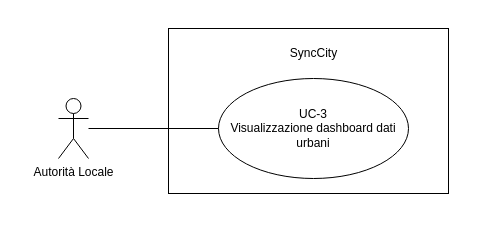
\includegraphics[width=0.6\textwidth]{analisi_dei_requisiti/UC-3.png}
	\captionof{figure}{UC-3: Visualizzazione \href{https://7last.github.io/docs/rtb/documentazione-interna/glossario\#dashboard}{dashboard\textsubscript{G}} \href{https://7last.github.io/docs/rtb/documentazione-interna/glossario\#dati-urbani}{dati urbani\textsubscript{G}}}
\end{center}

\subsubsubsubsection{UC-3.1: Visualizzazione grafico time series per traffico giornaliero}
\begin{itemize}
	\item \textbf{Attore principale}: Autorità locale;
	\item \textbf{Precondizioni}:
	      \begin{enumerate}
		      \item L'autorità locale ha effettuato l'accesso al sistema ed esso è in funzione;
		      \item Il sistema ha caricato la \href{https://7last.github.io/docs/rtb/documentazione-interna/glossario\#dashboard}{dashboard\textsubscript{G}} relativa ai \href{https://7last.github.io/docs/rtb/documentazione-interna/glossario\#dati-atmosferici}{dati atmosferici\textsubscript{G}};
	      \end{enumerate}
	\item \textbf{Postcondizioni}: L'autorità locale visualizza un grafico contenente le misurazioni storiche del traffico giornaliero;
	\item \textbf{Scenario principale}:
	      \begin{enumerate}
		      \item L'autorità locale accede alla piattaforma;
		      \item Il sistema carica i dati relativi ai sensori interrogando il database;
		      \item L'autorità locale seleziona la visualizzazione della \href{https://7last.github.io/docs/rtb/documentazione-interna/glossario\#dashboard}{dashboard\textsubscript{G}} relativa ai \href{https://7last.github.io/docs/rtb/documentazione-interna/glossario\#dati-urbani}{dati urbani\textsubscript{G}}.
	      \end{enumerate}
	\item \href{https://7last.github.io/docs/rtb/documentazione-interna/glossario\#user-story}{\textbf{User story}\textsubscript{G}}:
	      Come autorità locale desidero poter visualizzare un grafico \href{https://7last.github.io/docs/rtb/documentazione-interna/glossario\#time-series}{time series\textsubscript{G}} contenente le misurazioni storiche del traffico giornaliero
	      per poter monitorarne l'andamento nel tempo e facilmente individuare eventuali anomalie.
\end{itemize}

\begin{center}
	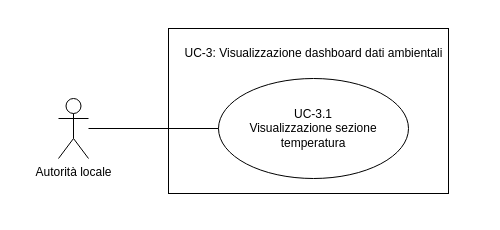
\includegraphics[width=0.6\textwidth]{analisi_dei_requisiti/UC-3.1.png}
	\captionof{figure}{UC-3.1: Visualizzazione grafico \href{https://7last.github.io/docs/rtb/documentazione-interna/glossario\#time-series}{time series\textsubscript{G}} per traffico giornaliero}
\end{center}
\subsubsubsubsection{UC-3.2: Visualizzazione mappa interattiva traffico in tempo reale}
\begin{itemize}
	\item \textbf{Attore principale}: Autorità locale;
	\item \textbf{Precondizioni}:
	      \begin{enumerate}
		      \item L'autorità locale ha effettuato l'accesso al sistema ed esso è in funzione;
		      \item Il sistema ha caricato la \href{https://7last.github.io/docs/rtb/documentazione-interna/glossario\#dashboard}{dashboard\textsubscript{G}} relativa ai \href{https://7last.github.io/docs/rtb/documentazione-interna/glossario\#dati-atmosferici}{dati atmosferici\textsubscript{G}};
	      \end{enumerate}
	\item \textbf{Postcondizioni}: L'autorità locale visualizza una mappa interattiva contenente i dati relativi al traffico in tempo reale;
	\item \textbf{Scenario principale}:
	      \begin{enumerate}
		      \item L'autorità locale accede alla piattaforma;
		      \item Il sistema carica i dati relativi ai sensori interrogando il database;
		      \item L'autorità locale seleziona la visualizzazione della \href{https://7last.github.io/docs/rtb/documentazione-interna/glossario\#dashboard}{dashboard\textsubscript{G}} relativa ai \href{https://7last.github.io/docs/rtb/documentazione-interna/glossario\#dati-urbani}{dati urbani\textsubscript{G}}.
	      \end{enumerate}
	\item \href{https://7last.github.io/docs/rtb/documentazione-interna/glossario\#user-story}{\textbf{User story}\textsubscript{G}}: Come autorità locale desidero poter visualizzare una mappa interattiva contenente i dati relativi al traffico in tempo reale
	      per poter monitorare l'andamento del traffico e prendere decisioni in base ad esso.
\end{itemize}

\begin{center}
	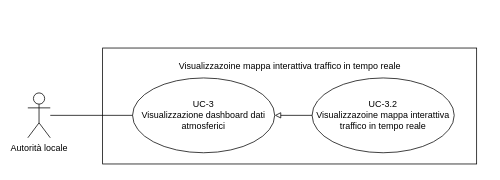
\includegraphics[width=0.6\textwidth]{analisi_dei_requisiti/UC-3.2.png}
	\captionof{figure}{UC-3.2: Visualizzazione mappa interattiva traffico in tempo reale}
\end{center}

\subsubsubsubsection{UC-3.3: Visualizzazione mappa interattiva lavori in corso}
\begin{itemize}
	\item \textbf{Attore principale}: Autorità locale;
	\item \textbf{Precondizioni}:
	      \begin{enumerate}
		      \item L'autorità locale ha effettuato l'accesso al sistema ed esso è in funzione;
		      \item Il sistema ha caricato la \href{https://7last.github.io/docs/rtb/documentazione-interna/glossario\#dashboard}{dashboard\textsubscript{G}} relativa ai \href{https://7last.github.io/docs/rtb/documentazione-interna/glossario\#dati-atmosferici}{dati atmosferici\textsubscript{G}};
	      \end{enumerate}
	\item \textbf{Postcondizioni}: L'autorità locale visualizza una mappa interattiva contenente i dati relativi ai lavori in corso;
	\item \textbf{Scenario principale}:
	      \begin{enumerate}
		      \item L'autorità locale accede alla piattaforma;
		      \item Il sistema carica i dati relativi ai sensori interrogando il database;
		      \item L'autorità locale seleziona la visualizzazione della \href{https://7last.github.io/docs/rtb/documentazione-interna/glossario\#dashboard}{dashboard\textsubscript{G}} relativa ai \href{https://7last.github.io/docs/rtb/documentazione-interna/glossario\#dati-urbani}{dati urbani\textsubscript{G}}.
	      \end{enumerate}
	\item \href{https://7last.github.io/docs/rtb/documentazione-interna/glossario\#user-story}{\textbf{User story}\textsubscript{G}}:
	      Come autorità locale desidero poter visualizzare una mappa interattiva contenente i dati relativi ai lavori in corso
	      per poterne monitorare la posizione, lo stato e prendere decisioni in base ad essi.
\end{itemize}

\begin{center}
	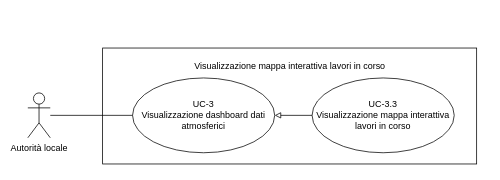
\includegraphics[width=0.6\textwidth]{analisi_dei_requisiti/UC-3.3.png}
	\captionof{figure}{UC-3.3: Visualizzazione mappa interattiva lavori in corso}
\end{center}

\subsubsubsubsection{UC-3.4: Visualizzazione grafico time series per incidenti}
\begin{itemize}
	\item \textbf{Attore principale}: Autorità locale;
	\item \textbf{Precondizioni}:
	      \begin{enumerate}
		      \item L'autorità locale ha effettuato l'accesso al sistema ed esso è in funzione;
		      \item Il sistema ha caricato la \href{https://7last.github.io/docs/rtb/documentazione-interna/glossario\#dashboard}{dashboard\textsubscript{G}} relativa ai \href{https://7last.github.io/docs/rtb/documentazione-interna/glossario\#dati-atmosferici}{dati atmosferici\textsubscript{G}};
	      \end{enumerate}
	\item \textbf{Postcondizioni}: L'autorità locale visualizza un grafico \href{https://7last.github.io/docs/rtb/documentazione-interna/glossario\#time-series}{time series\textsubscript{G}} contenente le misurazioni storiche degli incidenti;
	\item \textbf{Scenario principale}:
	      \begin{enumerate}
		      \item L'autorità locale accede alla piattaforma;
		      \item Il sistema carica i dati relativi ai sensori interrogando il database;
		      \item L'autorità locale seleziona la visualizzazione della \href{https://7last.github.io/docs/rtb/documentazione-interna/glossario\#dashboard}{dashboard\textsubscript{G}} relativa ai \href{https://7last.github.io/docs/rtb/documentazione-interna/glossario\#dati-urbani}{dati urbani\textsubscript{G}}.
	      \end{enumerate}
	\item \href{https://7last.github.io/docs/rtb/documentazione-interna/glossario\#user-story}{\textbf{User story}\textsubscript{G}}: Come autorità locale desidero poter visualizzare un grafico \href{https://7last.github.io/docs/rtb/documentazione-interna/glossario\#time-series}{time series\textsubscript{G}} contenente le misurazioni storiche degli incidenti
	      per poter monitorarne l'andamento nel tempo e facilmente individuare eventuali anomalie.
\end{itemize}

\begin{center}
	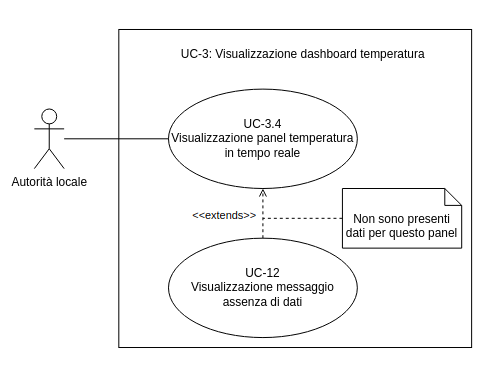
\includegraphics[width=0.6\textwidth]{analisi_dei_requisiti/UC-3.4.png}
	\captionof{figure}{UC-3.4: Visualizzazione grafico \href{https://7last.github.io/docs/rtb/documentazione-interna/glossario\#time-series}{time series\textsubscript{G}} per incidenti}
\end{center}
\subsubsubsubsection{UC-3.5: Visualizzazione mappa interattiva incidenti in tempo reale}
\begin{itemize}
	\item \textbf{Attore principale}: Autorità locale;
	\item \textbf{Precondizioni}:
	      \begin{enumerate}
		      \item L'autorità locale ha effettuato l'accesso al sistema ed esso è in funzione;
		      \item Il sistema ha caricato la \href{https://7last.github.io/docs/rtb/documentazione-interna/glossario\#dashboard}{dashboard\textsubscript{G}} relativa ai \href{https://7last.github.io/docs/rtb/documentazione-interna/glossario\#dati-atmosferici}{dati atmosferici\textsubscript{G}};
	      \end{enumerate}
	\item \textbf{Postcondizioni}: L'autorità locale visualizza una mappa interattiva contenente i dati relativi agli incidenti in tempo reale;
	\item \textbf{Scenario principale}:
	      \begin{enumerate}
		      \item L'autorità locale accede alla piattaforma;
		      \item Il sistema carica i dati relativi ai sensori interrogando il database;
		      \item L'autorità locale seleziona la visualizzazione della \href{https://7last.github.io/docs/rtb/documentazione-interna/glossario\#dashboard}{dashboard\textsubscript{G}} relativa ai \href{https://7last.github.io/docs/rtb/documentazione-interna/glossario\#dati-urbani}{dati urbani\textsubscript{G}}.
	      \end{enumerate}
	\item \href{https://7last.github.io/docs/rtb/documentazione-interna/glossario\#user-story}{\textbf{User story}\textsubscript{G}}: Come autorità locale desidero poter visualizzare una mappa interattiva contenente i dati relativi agli incidenti in tempo reale
	      per poter monitorare l'andamento degli incidenti e prendere decisioni in base ad essi.
\end{itemize}

\begin{center}
	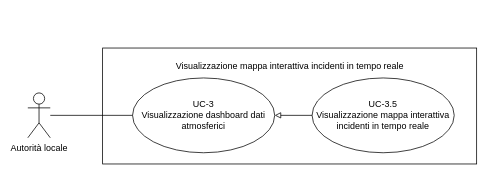
\includegraphics[width=0.6\textwidth]{analisi_dei_requisiti/UC-3.5.png}
	\captionof{figure}{UC-3.5: Visualizzazione mappa interattiva incidenti in tempo reale}
\end{center}
\subsubsubsubsection{UC-3.6: Visualizzazione \textit{panel} incidenti nell'ultimo mese}
\begin{itemize}
	\item \textbf{Attore principale}: Autorità locale;
	\item \textbf{Precondizioni}:
	      \begin{enumerate}
		      \item L'autorità locale ha effettuato l'accesso al sistema ed esso è in funzione;
		      \item Il sistema ha caricato la \href{https://7last.github.io/docs/rtb/documentazione-interna/glossario\#dashboard}{dashboard\textsubscript{G}} relativa ai \href{https://7last.github.io/docs/rtb/documentazione-interna/glossario\#dati-atmosferici}{dati atmosferici\textsubscript{G}};
	      \end{enumerate}
	\item \textbf{Postcondizioni}: L'autorità locale visualizza un \textit{panel} contenente il numero di incidenti avvenuti nell'ultimo mese;
	\item \textbf{Scenario principale}:
	      \begin{enumerate}
		      \item L'autorità locale accede alla piattaforma;
		      \item Il sistema carica i dati relativi ai sensori interrogando il database;
		      \item L'autorità locale seleziona la visualizzazione della \href{https://7last.github.io/docs/rtb/documentazione-interna/glossario\#dashboard}{dashboard\textsubscript{G}} relativa ai \href{https://7last.github.io/docs/rtb/documentazione-interna/glossario\#dati-urbani}{dati urbani\textsubscript{G}}.
	      \end{enumerate}
	\item \href{https://7last.github.io/docs/rtb/documentazione-interna/glossario\#user-story}{\textbf{User story}\textsubscript{G}}: Come autorità locale desidero poter visualizzare il numero di incidenti avvenuti nell'ultimo mese
	      per poterne monitorare l'andamento e prendere decisioni in base ad essi.
\end{itemize}

\begin{center}
	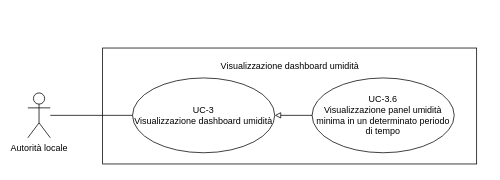
\includegraphics[width=0.6\textwidth]{analisi_dei_requisiti/UC-3.6.png}
	\captionof{figure}{UC-3.6: Visualizzazione \textit{panel} incidenti nell'ultimo mese}
\end{center}
\subsubsubsubsection{UC-3.7: Visualizzazione \textit{panel} incidenti nell'ultimo anno}
\begin{itemize}
	\item \textbf{Attore principale}: Autorità locale;
	\item \textbf{Precondizioni}:
	      \begin{enumerate}
		      \item L'autorità locale ha effettuato l'accesso al sistema ed esso è in funzione;
		      \item Il sistema ha caricato la \href{https://7last.github.io/docs/rtb/documentazione-interna/glossario\#dashboard}{dashboard\textsubscript{G}} relativa ai \href{https://7last.github.io/docs/rtb/documentazione-interna/glossario\#dati-atmosferici}{dati atmosferici\textsubscript{G}};
	      \end{enumerate}
	\item \textbf{Postcondizioni}: L'autorità locale visualizza un \textit{panel} contenente il numero di incidenti avvenuti nell'ultimo anno;
	\item \textbf{Scenario principale}:
	      \begin{enumerate}
		      \item L'autorità locale accede alla piattaforma;
		      \item Il sistema carica i dati relativi ai sensori interrogando il database;
		      \item L'autorità locale seleziona la visualizzazione della \href{https://7last.github.io/docs/rtb/documentazione-interna/glossario\#dashboard}{dashboard\textsubscript{G}} relativa ai \href{https://7last.github.io/docs/rtb/documentazione-interna/glossario\#dati-urbani}{dati urbani\textsubscript{G}}.
	      \end{enumerate}
	\item \href{https://7last.github.io/docs/rtb/documentazione-interna/glossario\#user-story}{\textbf{User story}\textsubscript{G}}: Come autorità locale desidero poter visualizzare il numero di incidenti avvenuti nell'ultimo anno
	      per poterne monitorare l'andamento e prendere decisioni in base ad essi.
\end{itemize}

\begin{center}
	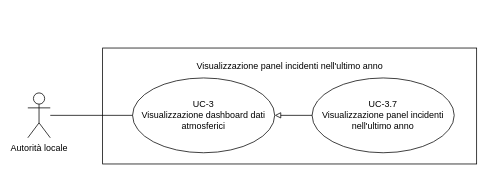
\includegraphics[width=0.6\textwidth]{analisi_dei_requisiti/UC-3.7.png}
	\captionof{figure}{UC-3.7: Visualizzazione \textit{panel} incidenti nell'ultimo anno}
\end{center}

\subsubsubsubsection{UC-3.8: Visualizzazione mappa interattiva colonnine di ricarica con stato di funzionamento}
\begin{itemize}
	\item \textbf{Attore principale}: Autorità locale;
	\item \textbf{Precondizioni}:
	      \begin{enumerate}
		      \item L'autorità locale ha effettuato l'accesso al sistema ed esso è in funzione;
		      \item Il sistema ha caricato la \href{https://7last.github.io/docs/rtb/documentazione-interna/glossario\#dashboard}{dashboard\textsubscript{G}} relativa ai \href{https://7last.github.io/docs/rtb/documentazione-interna/glossario\#dati-atmosferici}{dati atmosferici\textsubscript{G}};
	      \end{enumerate}
	\item \textbf{Postcondizioni}: L'autorità locale visualizza una mappa interattiva contenente le colonnine di ricarica con lo stato di funzionamento
	      di ognuna di esse;
	\item \textbf{Scenario principale}:
	      \begin{enumerate}
		      \item L'autorità locale accede alla piattaforma;
		      \item Il sistema carica i dati relativi ai sensori interrogando il database;
		      \item L'autorità locale seleziona la visualizzazione della \href{https://7last.github.io/docs/rtb/documentazione-interna/glossario\#dashboard}{dashboard\textsubscript{G}} relativa ai \href{https://7last.github.io/docs/rtb/documentazione-interna/glossario\#dati-urbani}{dati urbani\textsubscript{G}}.
	      \end{enumerate}
	\item \href{https://7last.github.io/docs/rtb/documentazione-interna/glossario\#user-story}{\textbf{User story}\textsubscript{G}}: Come autorità locale desidero poter visualizzare una mappa interattiva contenente le colonnine di ricarica con lo stato di funzionamento
	      di ognuna di esse per poterne monitorare lo stato e prendere decisioni in base ad esso.
\end{itemize}

\begin{center}
	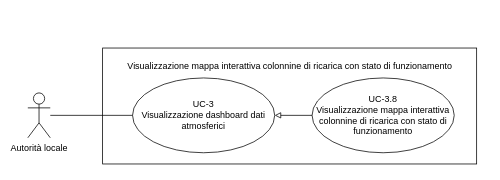
\includegraphics[width=0.6\textwidth]{analisi_dei_requisiti/UC-3.8.png}
	\captionof{figure}{UC-3.8: Visualizzazione mappa interattiva colonnine di ricarica con stato di funzionamento}
\end{center}
\subsubsubsubsection{UC-3.9: Visualizzazione \textit{panel} con conteggio colonnine guaste e funzionanti}
\begin{itemize}
	\item \textbf{Attore principale}: Autorità locale;
	\item \textbf{Precondizioni}:
	      \begin{enumerate}
		      \item L'autorità locale ha effettuato l'accesso al sistema ed esso è in funzione;
		      \item Il sistema ha caricato la \href{https://7last.github.io/docs/rtb/documentazione-interna/glossario\#dashboard}{dashboard\textsubscript{G}} relativa ai \href{https://7last.github.io/docs/rtb/documentazione-interna/glossario\#dati-atmosferici}{dati atmosferici\textsubscript{G}};
	      \end{enumerate}
	\item \textbf{Postcondizioni}: L'autorità locale visualizza un \textit{panel} contenente il conteggio delle colonnine di ricarica guaste e funzionanti;
	\item \textbf{Scenario principale}:
	      \begin{enumerate}
		      \item L'autorità locale accede alla piattaforma;
		      \item Il sistema carica i dati relativi ai sensori interrogando il database;
		      \item L'autorità locale seleziona la visualizzazione della \href{https://7last.github.io/docs/rtb/documentazione-interna/glossario\#dashboard}{dashboard\textsubscript{G}} relativa ai \href{https://7last.github.io/docs/rtb/documentazione-interna/glossario\#dati-urbani}{dati urbani\textsubscript{G}}.
	      \end{enumerate}
	\item \href{https://7last.github.io/docs/rtb/documentazione-interna/glossario\#user-story}{\textbf{User story}\textsubscript{G}}: Come autorità locale desidero poter visualizzare un \textit{panel} contenente il conteggio delle colonnine di ricarica guaste e funzionanti
	      per poterne monitorare lo stato e prendere decisioni in base ad esso.
\end{itemize}

\begin{center}
	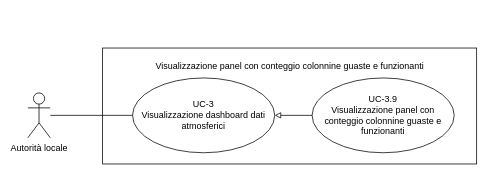
\includegraphics[width=0.6\textwidth]{analisi_dei_requisiti/UC-3.9.png}
	\captionof{figure}{UC-3.9: Visualizzazione \textit{panel} con conteggio colonnine guaste e funzionanti}
\end{center}

\subsubsubsubsection{UC-3.10: Visualizzazione mappa interattiva isole ecologiche con stato di riempimento}
\begin{itemize}
	\item \textbf{Attore principale}: Autorità locale;
	\item \textbf{Precondizioni}:
	      \begin{enumerate}
		      \item L'autorità locale ha effettuato l'accesso al sistema ed esso è in funzione;
		      \item Il sistema ha caricato la \href{https://7last.github.io/docs/rtb/documentazione-interna/glossario\#dashboard}{dashboard\textsubscript{G}} relativa ai \href{https://7last.github.io/docs/rtb/documentazione-interna/glossario\#dati-atmosferici}{dati atmosferici\textsubscript{G}};
	      \end{enumerate}
	\item \textbf{Postcondizioni}: L'autorità locale visualizza una mappa interattiva contenente le isole ecologiche con lo stato di riempimento
	      di ognuna di esse;
	\item \textbf{Scenario principale}:
	      \begin{enumerate}
		      \item L'autorità locale accede alla piattaforma;
		      \item Il sistema carica i dati relativi ai sensori interrogando il database;
		      \item L'autorità locale seleziona la visualizzazione della \href{https://7last.github.io/docs/rtb/documentazione-interna/glossario\#dashboard}{dashboard\textsubscript{G}} relativa ai \href{https://7last.github.io/docs/rtb/documentazione-interna/glossario\#dati-urbani}{dati urbani\textsubscript{G}}.
	      \end{enumerate}
	\item \href{https://7last.github.io/docs/rtb/documentazione-interna/glossario\#user-story}{\textbf{User story}\textsubscript{G}}: Come autorità locale desidero poter visualizzare una mappa interattiva contenente le isole ecologiche con lo stato di riempimento
	      di ognuna di esse per poterne monitorare lo stato e prendere decisioni in base ad esso.
\end{itemize}

\begin{center}
	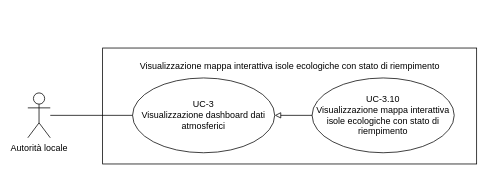
\includegraphics[width=0.6\textwidth]{analisi_dei_requisiti/UC-3.10.png}
	\captionof{figure}{UC-3.10: Visualizzazione mappa interattiva isole ecologiche con stato di riempimento}
\end{center}
\subsubsubsubsection{UC-3.11: Visualizzazione \textit{panel} con conteggio isole piene}
\begin{itemize}
	\item \textbf{Attore principale}: Autorità locale;
	\item \textbf{Precondizioni}:
	      \begin{enumerate}
		      \item L'autorità locale ha effettuato l'accesso al sistema ed esso è in funzione;
		      \item Il sistema ha caricato la \href{https://7last.github.io/docs/rtb/documentazione-interna/glossario\#dashboard}{dashboard\textsubscript{G}} relativa ai \href{https://7last.github.io/docs/rtb/documentazione-interna/glossario\#dati-atmosferici}{dati atmosferici\textsubscript{G}};
	      \end{enumerate}
	\item \textbf{Postcondizioni}: L'autorità locale visualizza un \textit{panel} contenente il conteggio delle isole ecologiche piene;
	\item \textbf{Scenario principale}:
	      \begin{enumerate}
		      \item L'autorità locale accede alla piattaforma;
		      \item Il sistema carica i dati relativi ai sensori interrogando il database;
		      \item L'autorità locale seleziona la visualizzazione della \href{https://7last.github.io/docs/rtb/documentazione-interna/glossario\#dashboard}{dashboard\textsubscript{G}} relativa ai \href{https://7last.github.io/docs/rtb/documentazione-interna/glossario\#dati-urbani}{dati urbani\textsubscript{G}}.
	      \end{enumerate}
	\item \href{https://7last.github.io/docs/rtb/documentazione-interna/glossario\#user-story}{\textbf{User story}\textsubscript{G}}: Come autorità locale desidero poter visualizzare un \textit{panel} contenente il conteggio delle isole ecologiche piene
	      per poterne monitorare lo stato e prendere decisioni in base ad esso.
\end{itemize}

\begin{center}
	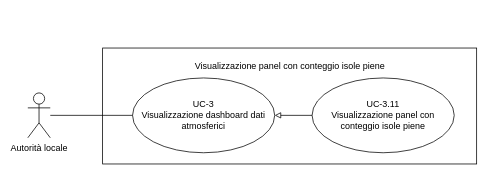
\includegraphics[width=0.6\textwidth]{analisi_dei_requisiti/UC-3.11.png}
	\captionof{figure}{UC-3.11: Visualizzazione \textit{panel} con conteggio isole piene}
\end{center}

\subsubsubsubsection{UC-3.12: Visualizzazione mappa interattiva parcheggi con rispettivo stato di occupazione}
\begin{itemize}
	\item \textbf{Attore principale}: Autorità locale;
	\item \textbf{Precondizioni}:
	      \begin{enumerate}
		      \item L'autorità locale ha effettuato l'accesso al sistema ed esso è in funzione;
		      \item Il sistema ha caricato la \href{https://7last.github.io/docs/rtb/documentazione-interna/glossario\#dashboard}{dashboard\textsubscript{G}} relativa ai \href{https://7last.github.io/docs/rtb/documentazione-interna/glossario\#dati-atmosferici}{dati atmosferici\textsubscript{G}};
	      \end{enumerate}
	\item \textbf{Postcondizioni}: L'autorità locale visualizza una mappa interattiva contenente i parcheggi con lo stato di occupazione
	      di ognuno di essi;
	\item \textbf{Scenario principale}:
	      \begin{enumerate}
		      \item L'autorità locale accede alla piattaforma;
		      \item Il sistema carica i dati relativi ai sensori interrogando il database;
		      \item L'autorità locale seleziona la visualizzazione della \href{https://7last.github.io/docs/rtb/documentazione-interna/glossario\#dashboard}{dashboard\textsubscript{G}} relativa ai \href{https://7last.github.io/docs/rtb/documentazione-interna/glossario\#dati-urbani}{dati urbani\textsubscript{G}}.
	      \end{enumerate}
	\item \href{https://7last.github.io/docs/rtb/documentazione-interna/glossario\#user-story}{\textbf{User story}\textsubscript{G}}: Come autorità locale desidero poter visualizzare una mappa interattiva contenente i parcheggi con lo stato di occupazione
	      di ognuno di essi.
\end{itemize}

\begin{center}
	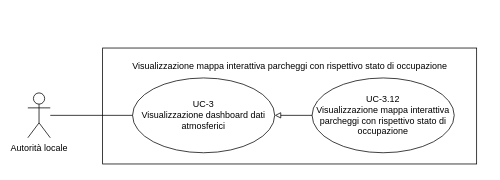
\includegraphics[width=0.6\textwidth]{analisi_dei_requisiti/UC-3.12.png}
	\captionof{figure}{UC-3.12: Visualizzazione mappa interattiva parcheggi con rispettivo stato di occupazione}
\end{center}
\subsubsubsubsection{UC-3.13: Visualizzazione \textit{panel} con conteggio parcheggi occupati e liberi}
\begin{itemize}
	\item \textbf{Attore principale}: Autorità locale;
	\item \textbf{Precondizioni}:
	      \begin{enumerate}
		      \item L'autorità locale ha effettuato l'accesso al sistema ed esso è in funzione;
		      \item Il sistema ha caricato la \href{https://7last.github.io/docs/rtb/documentazione-interna/glossario\#dashboard}{dashboard\textsubscript{G}} relativa ai \href{https://7last.github.io/docs/rtb/documentazione-interna/glossario\#dati-atmosferici}{dati atmosferici\textsubscript{G}};
	      \end{enumerate}
	\item \textbf{Postcondizioni}: L'autorità locale visualizza un \textit{panel} contenente il conteggio dei parcheggi occupati e liberi;
	\item \textbf{Scenario principale}:
	      \begin{enumerate}
		      \item L'autorità locale accede alla piattaforma;
		      \item Il sistema carica i dati relativi ai sensori interrogando il database;
		      \item L'autorità locale seleziona la visualizzazione della \href{https://7last.github.io/docs/rtb/documentazione-interna/glossario\#dashboard}{dashboard\textsubscript{G}} relativa ai \href{https://7last.github.io/docs/rtb/documentazione-interna/glossario\#dati-urbani}{dati urbani\textsubscript{G}}.
	      \end{enumerate}
	\item \href{https://7last.github.io/docs/rtb/documentazione-interna/glossario\#user-story}{\textbf{User story}\textsubscript{G}}: Come autorità locale desidero poter visualizzare un \textit{panel} contenente il conteggio dei parcheggi occupati e liberi
	      per poterne monitorare lo stato.
\end{itemize}

\begin{center}
	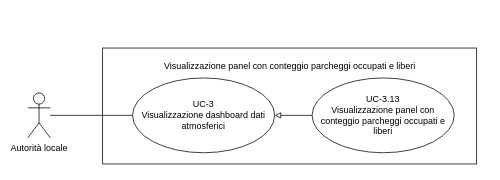
\includegraphics[width=0.6\textwidth]{analisi_dei_requisiti/UC-3.13.png}
	\captionof{figure}{UC-3.13: Visualizzazione \textit{panel} con conteggio parcheggi occupati e liberi}
\end{center}

\subsubsubsubsection{UC-3.14: Visualizzazione grafico time series per livello di acqua}
\begin{itemize}
	\item \textbf{Attore principale}: Autorità locale;
	\item \textbf{Precondizioni}:
	      \begin{enumerate}
		      \item L'autorità locale ha effettuato l'accesso al sistema ed esso è in funzione;
		      \item Il sistema ha caricato la \href{https://7last.github.io/docs/rtb/documentazione-interna/glossario\#dashboard}{dashboard\textsubscript{G}} relativa ai \href{https://7last.github.io/docs/rtb/documentazione-interna/glossario\#dati-atmosferici}{dati atmosferici\textsubscript{G}};
	      \end{enumerate}
	\item \textbf{Postcondizioni}: L'autorità locale visualizza un grafico \href{https://7last.github.io/docs/rtb/documentazione-interna/glossario\#time-series}{time series\textsubscript{G}} contenente le misurazioni storiche del livello di acqua;
	\item \textbf{Scenario principale}:
	      \begin{enumerate}
		      \item L'autorità locale accede alla piattaforma;
		      \item Il sistema carica i dati relativi ai sensori interrogando il database;
		      \item L'autorità locale seleziona la visualizzazione della \href{https://7last.github.io/docs/rtb/documentazione-interna/glossario\#dashboard}{dashboard\textsubscript{G}} relativa ai \href{https://7last.github.io/docs/rtb/documentazione-interna/glossario\#dati-urbani}{dati urbani\textsubscript{G}}.
	      \end{enumerate}
	\item \href{https://7last.github.io/docs/rtb/documentazione-interna/glossario\#user-story}{\textbf{User story}\textsubscript{G}}: Come autorità locale desidero poter visualizzare un grafico \href{https://7last.github.io/docs/rtb/documentazione-interna/glossario\#time-series}{time series\textsubscript{G}} contenente le misurazioni storiche del livello di acqua
	      per poterne monitorarne l'andamento nel tempo e facilmente individuare eventuali anomalie.
\end{itemize}

\begin{center}
	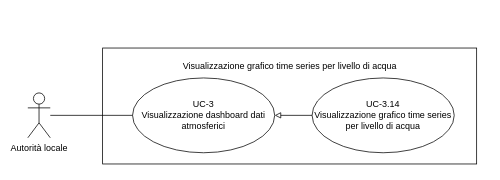
\includegraphics[width=0.6\textwidth]{analisi_dei_requisiti/UC-3.14.png}
	\captionof{figure}{UC-3.14: Visualizzazione grafico \href{https://7last.github.io/docs/rtb/documentazione-interna/glossario\#time-series}{time series\textsubscript{G}} per livello di acqua}
\end{center}

\subsubsection{UC-4: Visualizzazione dashboard misurazioni anomale}
\begin{itemize}
	\item \textbf{Attore principale}: Autorità locale;
	\item \textbf{Precondizioni}:
	      \begin{enumerate}
		      \item L'autorità locale accede alla piattaforma;
		      \item Il sistema carica i dati relativi ai sensori interrogando il database;
	      \end{enumerate}
	\item \textbf{Postcondizioni}: L'autorità locale visualizza una \href{https://7last.github.io/docs/rtb/documentazione-interna/glossario\#dashboard}{dashboard\textsubscript{G}} contenente le misurazioni anomale effettuate dai sensori;
	\item \textbf{Scenario principale}:
	      \begin{enumerate}
		      \item L'autorità locale accede alla piattaforma;
		      \item Il sistema carica i dati relativi ai sensori interrogando il database;
		      \item L'autorità locale seleziona la visualizzazione della \href{https://7last.github.io/docs/rtb/documentazione-interna/glossario\#dashboard}{dashboard\textsubscript{G}} relativa alle misurazioni anomale.
	      \end{enumerate}
	\item \href{https://7last.github.io/docs/rtb/documentazione-interna/glossario\#user-story}{\textbf{User story}\textsubscript{G}}: Come autorità locale desidero poter visualizzare le misurazioni anomale effettuate dai sensori
	      per poterne monitorare l'andamento e prendere decisioni in base ad esse.
\end{itemize}

\begin{center}
	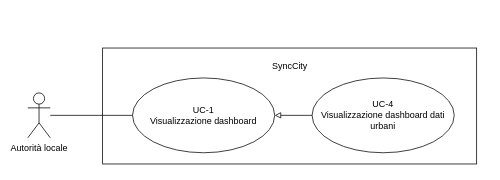
\includegraphics[width=0.6\textwidth]{analisi_dei_requisiti/UC-4.png}
	\captionof{figure}{UC-4: Visualizzazione \href{https://7last.github.io/docs/rtb/documentazione-interna/glossario\#dashboard}{dashboard\textsubscript{G}} misurazioni anomale}
\end{center}

\subsubsection{UC-5: Visualizzazione con filtri}
\begin{itemize}
	\item \textbf{Attore principale}: Autorità locale;
	\item \textbf{Precondizioni}:
	\item \textbf{Postcondizioni}:
	\item \textbf{Scenario principale}:
	\item \href{https://7last.github.io/docs/rtb/documentazione-interna/glossario\#user-story}{\textbf{User story}\textsubscript{G}}: Come autorità locale desidero poter visualizzare i \href{https://7last.github.io/docs/rtb/documentazione-interna/glossario\#dati-urbani}{dati urbani\textsubscript{G}} con filtri
	      per poter monitorare solo i dati che mi interessano e prendere decisioni in base ad essi.

\end{itemize}

\begin{center}
	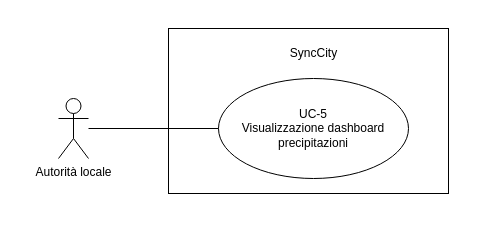
\includegraphics[width=0.6\textwidth]{analisi_dei_requisiti/UC-5.png}
	\captionof{figure}{UC-5: Visualizzazione con filtri}
\end{center}

% TODO: sottocasi di UC-6

\subsubsection{UC-6: Visualizzazione messaggio assenza di dati}
\begin{itemize}
	\item \textbf{Attore principale}: Autorità locale;
	\item \textbf{Precondizioni}:
	      \begin{enumerate}
		      \item L'autorità locale accede alla piattaforma;
		      \item Il sistema carica i dati relativi ai sensori interrogando il database;
	      \end{enumerate}
	\item \textbf{Postcondizioni}: L'autorità locale visualizza un messaggio che notifica l'assenza di dati;
	\item \textbf{Scenario principale}:
	      \begin{enumerate}
		      \item L'autorità locale accede alla piattaforma;
		      \item Il sistema carica i dati relativi ai sensori interrogando il database;
		      \item Il sistema non trova dati relativi ai sensori;
		      \item Il sistema mostra un messaggio che notifica l'assenza di dati.
	      \end{enumerate}
\end{itemize}

\begin{center}
	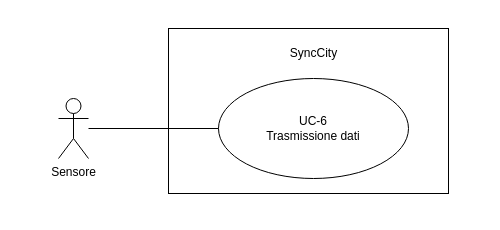
\includegraphics[width=0.6\textwidth]{analisi_dei_requisiti/UC-6.png}
	\captionof{figure}{UC-6: Visualizzazione messaggio assenza di dati}
\end{center}

\subsubsection{UC-7: Trasmissione dati temperatura}
\begin{itemize}
	\item \textbf{Attore principale}: \href{https://7last.github.io/docs/rtb/documentazione-interna/glossario\#sensore}{Sensore\textsubscript{G}};
	\item \textbf{Precondizioni}: Il \href{https://7last.github.io/docs/rtb/documentazione-interna/glossario\#sensore}{sensore\textsubscript{G}} è attivo e collegato al sistema;
	\item \textbf{Postcondizioni}: I dati inviati dal \href{https://7last.github.io/docs/rtb/documentazione-interna/glossario\#sensore}{sensore\textsubscript{G}} sono stati elaborati e memorizzati nel sistema;
	\item \textbf{Scenario principale}:
	      \begin{enumerate}
		      \item Il \href{https://7last.github.io/docs/rtb/documentazione-interna/glossario\#sensore}{sensore\textsubscript{G}} effettua una misurazione di temperatura;
		      \item Il \href{https://7last.github.io/docs/rtb/documentazione-interna/glossario\#sensore}{sensore\textsubscript{G}} formatta i dati da inviare al sistema, includendo oltre alle misurazioni l'identificativo del \href{https://7last.github.io/docs/rtb/documentazione-interna/glossario\#sensore}{sensore\textsubscript{G}},
		            il timestamp, e la sua posizione geografica;
		      \item Il \href{https://7last.github.io/docs/rtb/documentazione-interna/glossario\#sensore}{sensore\textsubscript{G}} invia i dati al sistema.
	      \end{enumerate}
	\item \href{https://7last.github.io/docs/rtb/documentazione-interna/glossario\#user-story}{\textbf{User story}\textsubscript{G}}: Come \href{https://7last.github.io/docs/rtb/documentazione-interna/glossario\#sensore}{sensore\textsubscript{G}}, desidero poter inviare al sistema le rilevazioni della temperatura.
\end{itemize}

\begin{center}
	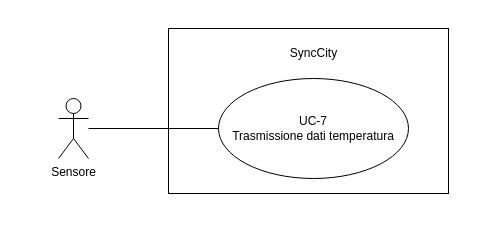
\includegraphics[width=0.6\textwidth]{analisi_dei_requisiti/UC-7.png}
	\captionof{figure}{UC-7: Trasmissione dati temperatura}
\end{center}

\subsubsection{UC-8: Trasmissione dati umidità}
\begin{itemize}
	\item \textbf{Attore principale}: \href{https://7last.github.io/docs/rtb/documentazione-interna/glossario\#sensore}{Sensore\textsubscript{G}};
	\item \textbf{Precondizioni}: Il \href{https://7last.github.io/docs/rtb/documentazione-interna/glossario\#sensore}{sensore\textsubscript{G}} è attivo e collegato al sistema;
	\item \textbf{Postcondizioni}: I dati inviati dal \href{https://7last.github.io/docs/rtb/documentazione-interna/glossario\#sensore}{sensore\textsubscript{G}} sono stati elaborati e memorizzati nel sistema;
	\item \textbf{Scenario principale}:
	      \begin{enumerate}
		      \item Il \href{https://7last.github.io/docs/rtb/documentazione-interna/glossario\#sensore}{sensore\textsubscript{G}} effettua una misurazione dell'umidità;
		      \item Il \href{https://7last.github.io/docs/rtb/documentazione-interna/glossario\#sensore}{sensore\textsubscript{G}} formatta i dati da inviare al sistema, includendo oltre alle misurazioni l'identificativo del \href{https://7last.github.io/docs/rtb/documentazione-interna/glossario\#sensore}{sensore\textsubscript{G}},
		            il timestamp, e la sua posizione geografica;
		      \item Il \href{https://7last.github.io/docs/rtb/documentazione-interna/glossario\#sensore}{sensore\textsubscript{G}} invia i dati al sistema.
	      \end{enumerate}
	\item \href{https://7last.github.io/docs/rtb/documentazione-interna/glossario\#user-story}{\textbf{User story}\textsubscript{G}}: Come \href{https://7last.github.io/docs/rtb/documentazione-interna/glossario\#sensore}{sensore\textsubscript{G}}, desidero poter inviare al sistema le rilevazioni dell'umidità.
\end{itemize}

\begin{center}
	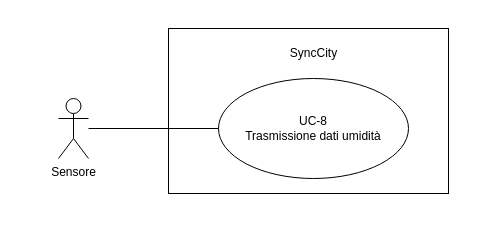
\includegraphics[width=0.6\textwidth]{analisi_dei_requisiti/UC-8.png}
	\captionof{figure}{UC-8: Trasmissione dati umidità}
\end{center}

\subsubsection{UC-9: Trasmissione dati pressione}
\begin{itemize}
	\item \textbf{Attore principale}: \href{https://7last.github.io/docs/rtb/documentazione-interna/glossario\#sensore}{Sensore\textsubscript{G}};
	\item \textbf{Precondizioni}: Il \href{https://7last.github.io/docs/rtb/documentazione-interna/glossario\#sensore}{sensore\textsubscript{G}} è attivo e collegato al sistema;
	\item \textbf{Postcondizioni}: I dati inviati dal \href{https://7last.github.io/docs/rtb/documentazione-interna/glossario\#sensore}{sensore\textsubscript{G}} sono stati elaborati e memorizzati nel sistema;
	\item \textbf{Scenario principale}:
	      \begin{enumerate}
		      \item Il \href{https://7last.github.io/docs/rtb/documentazione-interna/glossario\#sensore}{sensore\textsubscript{G}} effettua una misurazione della pressione;
		      \item Il \href{https://7last.github.io/docs/rtb/documentazione-interna/glossario\#sensore}{sensore\textsubscript{G}} formatta i dati da inviare al sistema, includendo oltre alle misurazioni l'identificativo del \href{https://7last.github.io/docs/rtb/documentazione-interna/glossario\#sensore}{sensore\textsubscript{G}},
		            il timestamp, e la sua posizione geografica;
		      \item Il \href{https://7last.github.io/docs/rtb/documentazione-interna/glossario\#sensore}{sensore\textsubscript{G}} invia i dati al sistema.
	      \end{enumerate}
	\item \href{https://7last.github.io/docs/rtb/documentazione-interna/glossario\#user-story}{\textbf{User story}\textsubscript{G}}: Come \href{https://7last.github.io/docs/rtb/documentazione-interna/glossario\#sensore}{sensore\textsubscript{G}}, desidero poter inviare al sistema le rilevazioni della pressione.
\end{itemize}

\begin{center}
	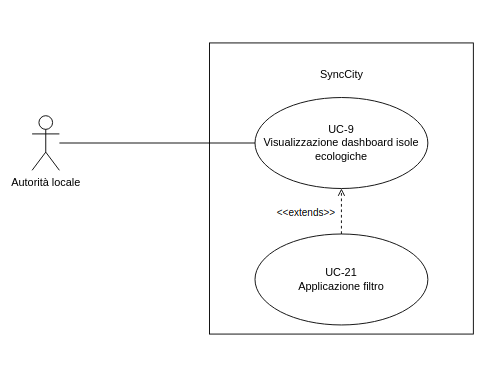
\includegraphics[width=0.6\textwidth]{analisi_dei_requisiti/UC-9.png}
	\captionof{figure}{UC-9: Trasmissione dati pressione}
\end{center}

\subsubsection{UC-10: Trasmissione dati precipitazioni}
\begin{itemize}
	\item \textbf{Attore principale}: \href{https://7last.github.io/docs/rtb/documentazione-interna/glossario\#sensore}{Sensore\textsubscript{G}};
	\item \textbf{Precondizioni}: Il \href{https://7last.github.io/docs/rtb/documentazione-interna/glossario\#sensore}{sensore\textsubscript{G}} è attivo e collegato al sistema;
	\item \textbf{Postcondizioni}: I dati inviati dal \href{https://7last.github.io/docs/rtb/documentazione-interna/glossario\#sensore}{sensore\textsubscript{G}} sono stati elaborati e memorizzati nel sistema;
	\item \textbf{Scenario principale}:
	      \begin{enumerate}
		      \item Il \href{https://7last.github.io/docs/rtb/documentazione-interna/glossario\#sensore}{sensore\textsubscript{G}} effettua una misurazione della quantità di precipitazioni;
		      \item Il \href{https://7last.github.io/docs/rtb/documentazione-interna/glossario\#sensore}{sensore\textsubscript{G}} formatta i dati da inviare al sistema, includendo oltre alle misurazioni l'identificativo del \href{https://7last.github.io/docs/rtb/documentazione-interna/glossario\#sensore}{sensore\textsubscript{G}},
		            il timestamp, e la sua posizione geografica;
		      \item Il \href{https://7last.github.io/docs/rtb/documentazione-interna/glossario\#sensore}{sensore\textsubscript{G}} invia i dati al sistema.
	      \end{enumerate}
	\item \href{https://7last.github.io/docs/rtb/documentazione-interna/glossario\#user-story}{\textbf{User story}\textsubscript{G}}: Come \href{https://7last.github.io/docs/rtb/documentazione-interna/glossario\#sensore}{sensore\textsubscript{G}}, desidero poter inviare al sistema le rilevazioni della quantità di precipitazioni.
\end{itemize}

\begin{center}
	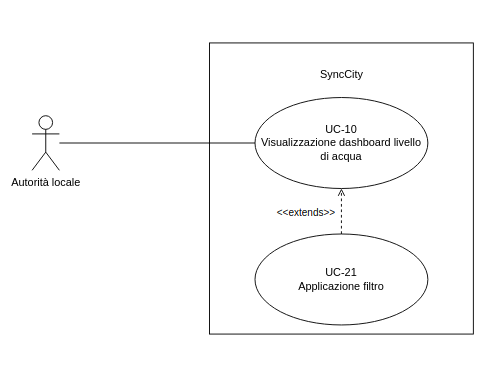
\includegraphics[width=0.6\textwidth]{analisi_dei_requisiti/UC-10.png}
	\captionof{figure}{UC-10: Trasmissione dati precipitazioni}
\end{center}

\subsubsection{UC-11: Trasmissione dati polveri sottili}
\begin{itemize}
	\item \textbf{Attore principale}: \href{https://7last.github.io/docs/rtb/documentazione-interna/glossario\#sensore}{Sensore\textsubscript{G}};
	\item \textbf{Precondizioni}: Il \href{https://7last.github.io/docs/rtb/documentazione-interna/glossario\#sensore}{sensore\textsubscript{G}} è attivo e collegato al sistema;
	\item \textbf{Postcondizioni}: I dati inviati dal \href{https://7last.github.io/docs/rtb/documentazione-interna/glossario\#sensore}{sensore\textsubscript{G}} sono stati elaborati e memorizzati nel sistema;
	\item \textbf{Scenario principale}:
	      \begin{enumerate}
		      \item Il \href{https://7last.github.io/docs/rtb/documentazione-interna/glossario\#sensore}{sensore\textsubscript{G}} effettua una misurazione della quantità di polveri sottili;
		      \item Il \href{https://7last.github.io/docs/rtb/documentazione-interna/glossario\#sensore}{sensore\textsubscript{G}} formatta i dati da inviare al sistema, includendo oltre alle misurazioni l'identificativo del \href{https://7last.github.io/docs/rtb/documentazione-interna/glossario\#sensore}{sensore\textsubscript{G}},
		            il timestamp, e la sua posizione geografica;
		      \item Il \href{https://7last.github.io/docs/rtb/documentazione-interna/glossario\#sensore}{sensore\textsubscript{G}} invia i dati al sistema.
	      \end{enumerate}
	\item \href{https://7last.github.io/docs/rtb/documentazione-interna/glossario\#user-story}{\textbf{User story}\textsubscript{G}}: Come \href{https://7last.github.io/docs/rtb/documentazione-interna/glossario\#sensore}{sensore\textsubscript{G}}, desidero poter inviare al sistema le rilevazioni della quantità di polveri sottili nell'aria.
\end{itemize}

\begin{center}
	\includegraphics[width=0.6\textwidth]{analisi_dei_requisiti/UC-11.png}
	\captionof{figure}{UC-11: Trasmissione dati polveri sottili}
\end{center}

\subsubsection{UC-12: Trasmissione dati traffico}
\begin{itemize}
	\item \textbf{Attore principale}: \href{https://7last.github.io/docs/rtb/documentazione-interna/glossario\#sensore}{Sensore\textsubscript{G}};
	\item \textbf{Precondizioni}: Il \href{https://7last.github.io/docs/rtb/documentazione-interna/glossario\#sensore}{sensore\textsubscript{G}} è attivo e collegato al sistema;
	\item \textbf{Postcondizioni}: I dati inviati dal \href{https://7last.github.io/docs/rtb/documentazione-interna/glossario\#sensore}{sensore\textsubscript{G}} sono stati elaborati e memorizzati nel sistema;
	\item \textbf{Scenario principale}:
	      \begin{enumerate}
		      \item Il \href{https://7last.github.io/docs/rtb/documentazione-interna/glossario\#sensore}{sensore\textsubscript{G}} effettua una misurazione del traffico;
		      \item Il \href{https://7last.github.io/docs/rtb/documentazione-interna/glossario\#sensore}{sensore\textsubscript{G}} formatta i dati da inviare al sistema, includendo oltre alle misurazioni l'identificativo del \href{https://7last.github.io/docs/rtb/documentazione-interna/glossario\#sensore}{sensore\textsubscript{G}},
		            il timestamp, e la sua posizione geografica;
		      \item Il \href{https://7last.github.io/docs/rtb/documentazione-interna/glossario\#sensore}{sensore\textsubscript{G}} invia i dati al sistema.
	      \end{enumerate}
	\item \href{https://7last.github.io/docs/rtb/documentazione-interna/glossario\#user-story}{\textbf{User story}\textsubscript{G}}: Come \href{https://7last.github.io/docs/rtb/documentazione-interna/glossario\#sensore}{sensore\textsubscript{G}}, desidero poter inviare al sistema le rilevazioni sui dati del traffico.
\end{itemize}

\begin{center}
	\includegraphics[width=0.6\textwidth]{analisi_dei_requisiti/UC-12.png}
	\captionof{figure}{UC-12: Trasmissione dati traffico}
\end{center}

\subsubsection{UC-13: Trasmissione dati lavori in corso}
\begin{itemize}
	\item \textbf{Attore principale}: \href{https://7last.github.io/docs/rtb/documentazione-interna/glossario\#sensore}{Sensore\textsubscript{G}};
	\item \textbf{Precondizioni}: Il \href{https://7last.github.io/docs/rtb/documentazione-interna/glossario\#sensore}{sensore\textsubscript{G}} è attivo e collegato al sistema;
	\item \textbf{Postcondizioni}: I dati inviati dal \href{https://7last.github.io/docs/rtb/documentazione-interna/glossario\#sensore}{sensore\textsubscript{G}} sono stati elaborati e memorizzati nel sistema;
	\item \textbf{Scenario principale}:
	      \begin{enumerate}
		      \item Il \href{https://7last.github.io/docs/rtb/documentazione-interna/glossario\#sensore}{sensore\textsubscript{G}} effettua una misurazione di temperatura;
		      \item Il \href{https://7last.github.io/docs/rtb/documentazione-interna/glossario\#sensore}{sensore\textsubscript{G}} formatta i dati da inviare al sistema, includendo oltre alle misurazioni l'identificativo del \href{https://7last.github.io/docs/rtb/documentazione-interna/glossario\#sensore}{sensore\textsubscript{G}},
		            il timestamp, e la sua posizione geografica;
		      \item Il \href{https://7last.github.io/docs/rtb/documentazione-interna/glossario\#sensore}{sensore\textsubscript{G}} invia i dati al sistema.
	      \end{enumerate}
	\item \href{https://7last.github.io/docs/rtb/documentazione-interna/glossario\#user-story}{\textbf{User story}\textsubscript{G}}: Come \href{https://7last.github.io/docs/rtb/documentazione-interna/glossario\#sensore}{sensore\textsubscript{G}}, desidero poter inviare al sistema le rilevazioni sui dati dei lavori in corso.
\end{itemize}

\begin{center}
	\includegraphics[width=0.6\textwidth]{analisi_dei_requisiti/UC-13.png}
	\captionof{figure}{UC-13: Trasmissione dati lavori in corso}
\end{center}

\subsubsection{UC-14: Trasmissione dati colonnine di ricarica}
\begin{itemize}
	\item \textbf{Attore principale}: \href{https://7last.github.io/docs/rtb/documentazione-interna/glossario\#sensore}{Sensore\textsubscript{G}};
	\item \textbf{Precondizioni}: Il \href{https://7last.github.io/docs/rtb/documentazione-interna/glossario\#sensore}{sensore\textsubscript{G}} è attivo e collegato al sistema;
	\item \textbf{Postcondizioni}: I dati inviati dal \href{https://7last.github.io/docs/rtb/documentazione-interna/glossario\#sensore}{sensore\textsubscript{G}} sono stati elaborati e memorizzati nel sistema;
	\item \textbf{Scenario principale}:
	      \begin{enumerate}
		      \item Il \href{https://7last.github.io/docs/rtb/documentazione-interna/glossario\#sensore}{sensore\textsubscript{G}} effettua una misurazione dello stato e l'occupazione delle colonnine di ricarica;
		      \item Il \href{https://7last.github.io/docs/rtb/documentazione-interna/glossario\#sensore}{sensore\textsubscript{G}} formatta i dati da inviare al sistema, includendo oltre alle misurazioni l'identificativo del \href{https://7last.github.io/docs/rtb/documentazione-interna/glossario\#sensore}{sensore\textsubscript{G}},
		            il timestamp, e la sua posizione geografica;
		      \item Il \href{https://7last.github.io/docs/rtb/documentazione-interna/glossario\#sensore}{sensore\textsubscript{G}} invia i dati al sistema.
	      \end{enumerate}
	\item \href{https://7last.github.io/docs/rtb/documentazione-interna/glossario\#user-story}{\textbf{User story}\textsubscript{G}}: Come \href{https://7last.github.io/docs/rtb/documentazione-interna/glossario\#sensore}{sensore\textsubscript{G}}, desidero poter inviare al sistema le rilevazioni sullo stato e l'occupazione delle colonnine di ricarica.
\end{itemize}

\begin{center}
	\includegraphics[width=0.6\textwidth]{analisi_dei_requisiti/UC-14.png}
	\captionof{figure}{UC-14: Trasmissione dati colonnine di ricarica}
\end{center}

\subsubsection{UC-15: Trasmissione dati isole ecologiche}
\begin{itemize}
	\item \textbf{Attore principale}: \href{https://7last.github.io/docs/rtb/documentazione-interna/glossario\#sensore}{Sensore\textsubscript{G}};
	\item \textbf{Precondizioni}: Il \href{https://7last.github.io/docs/rtb/documentazione-interna/glossario\#sensore}{sensore\textsubscript{G}} è attivo e collegato al sistema;
	\item \textbf{Postcondizioni}: I dati inviati dal \href{https://7last.github.io/docs/rtb/documentazione-interna/glossario\#sensore}{sensore\textsubscript{G}} sono stati elaborati e memorizzati nel sistema;
	\item \textbf{Scenario principale}:
	      \begin{enumerate}
		      \item Il \href{https://7last.github.io/docs/rtb/documentazione-interna/glossario\#sensore}{sensore\textsubscript{G}} effettua una misurazione dello stato di riempimento delle isole ecologiche;
		      \item Il \href{https://7last.github.io/docs/rtb/documentazione-interna/glossario\#sensore}{sensore\textsubscript{G}} formatta i dati da inviare al sistema, includendo oltre alle misurazioni l'identificativo del \href{https://7last.github.io/docs/rtb/documentazione-interna/glossario\#sensore}{sensore\textsubscript{G}},
		            il timestamp, e la sua posizione geografica;
		      \item Il \href{https://7last.github.io/docs/rtb/documentazione-interna/glossario\#sensore}{sensore\textsubscript{G}} invia i dati al sistema.
	      \end{enumerate}
	\item \href{https://7last.github.io/docs/rtb/documentazione-interna/glossario\#user-story}{\textbf{User story}\textsubscript{G}}: Come \href{https://7last.github.io/docs/rtb/documentazione-interna/glossario\#sensore}{sensore\textsubscript{G}}, desidero poter inviare al sistema le rilevazioni sullo stato di riempimento delle isole ecologiche.
\end{itemize}

\begin{center}
	\includegraphics[width=0.6\textwidth]{analisi_dei_requisiti/UC-15.png}
	\captionof{figure}{UC-15: Trasmissione dati isole ecologiche}
\end{center}

\subsubsection{UC-16: Trasmissione dati parcheggi}
\begin{itemize}
	\item \textbf{Attore principale}: \href{https://7last.github.io/docs/rtb/documentazione-interna/glossario\#sensore}{Sensore\textsubscript{G}};
	\item \textbf{Precondizioni}: Il \href{https://7last.github.io/docs/rtb/documentazione-interna/glossario\#sensore}{sensore\textsubscript{G}} è attivo e collegato al sistema;
	\item \textbf{Postcondizioni}: I dati inviati dal \href{https://7last.github.io/docs/rtb/documentazione-interna/glossario\#sensore}{sensore\textsubscript{G}} sono stati elaborati e memorizzati nel sistema;
	\item \textbf{Scenario principale}:
	      \begin{enumerate}
		      \item Il \href{https://7last.github.io/docs/rtb/documentazione-interna/glossario\#sensore}{sensore\textsubscript{G}} effettua una misurazione dello stato di riempimento del parcheggio;
		      \item Il \href{https://7last.github.io/docs/rtb/documentazione-interna/glossario\#sensore}{sensore\textsubscript{G}} formatta i dati da inviare al sistema, includendo oltre alle misurazioni l'identificativo del \href{https://7last.github.io/docs/rtb/documentazione-interna/glossario\#sensore}{sensore\textsubscript{G}},
		            il timestamp, e la sua posizione geografica;
		      \item Il \href{https://7last.github.io/docs/rtb/documentazione-interna/glossario\#sensore}{sensore\textsubscript{G}} invia i dati al sistema.
	      \end{enumerate}
	\item \href{https://7last.github.io/docs/rtb/documentazione-interna/glossario\#user-story}{\textbf{User story}\textsubscript{G}}: Come \href{https://7last.github.io/docs/rtb/documentazione-interna/glossario\#sensore}{sensore\textsubscript{G}}, desidero poter inviare al sistema le rilevazioni sull'occupazione dei parcheggi.
\end{itemize}

\begin{center}
	\includegraphics[width=0.6\textwidth]{analisi_dei_requisiti/UC-16.png}
	\captionof{figure}{UC-16: Trasmissione dati parcheggi}
\end{center}

\subsubsection{UC-17: Trasmissione dati livello di acqua}
\begin{itemize}
	\item \textbf{Attore principale}: \href{https://7last.github.io/docs/rtb/documentazione-interna/glossario\#sensore}{Sensore\textsubscript{G}};
	\item \textbf{Precondizioni}: Il \href{https://7last.github.io/docs/rtb/documentazione-interna/glossario\#sensore}{sensore\textsubscript{G}} è attivo e collegato al sistema;
	\item \textbf{Postcondizioni}: I dati inviati dal \href{https://7last.github.io/docs/rtb/documentazione-interna/glossario\#sensore}{sensore\textsubscript{G}} sono stati elaborati e memorizzati nel sistema;
	\item \textbf{Scenario principale}:
	      \begin{enumerate}
		      \item Il \href{https://7last.github.io/docs/rtb/documentazione-interna/glossario\#sensore}{sensore\textsubscript{G}} effettua una misurazione del livello di acqua;
		      \item Il \href{https://7last.github.io/docs/rtb/documentazione-interna/glossario\#sensore}{sensore\textsubscript{G}} formatta i dati da inviare al sistema, includendo oltre alle misurazioni l'identificativo del \href{https://7last.github.io/docs/rtb/documentazione-interna/glossario\#sensore}{sensore\textsubscript{G}},
		            il timestamp, e la sua posizione geografica;
		      \item Il \href{https://7last.github.io/docs/rtb/documentazione-interna/glossario\#sensore}{sensore\textsubscript{G}} invia i dati al sistema.
	      \end{enumerate}
	\item \href{https://7last.github.io/docs/rtb/documentazione-interna/glossario\#user-story}{\textbf{User story}\textsubscript{G}}: Come \href{https://7last.github.io/docs/rtb/documentazione-interna/glossario\#sensore}{sensore\textsubscript{G}}, desidero poter inviare al sistema le rilevazioni sul livello di acqua.
\end{itemize}

\begin{center}
	\includegraphics[width=0.6\textwidth]{analisi_dei_requisiti/UC-17.png}
	\captionof{figure}{UC-17: Trasmissione dati livello di acqua}
\end{center}
